%%%%%%%%%%%%%%%%%%%%%%%%%%%%%%%%%%%%%%%%%
% Short Sectioned Assignment LaTeX Template Version 1.0 (5/5/12)
% This template has been downloaded from: http://www.LaTeXTemplates.com
% Original author:  Frits Wenneker (http://www.howtotex.com)
% License: CC BY-NC-SA 3.0 (http://creativecommons.org/licenses/by-nc-sa/3.0/)
%%%%%%%%%%%%%%%%%%%%%%%%%%%%%%%%%%%%%%%%%

% \documentclass[paper=a4, fontsize=11pt]{scrartcl} % A4 paper and 11pt font size
\documentclass[11pt, a4paper]{book}
\usepackage[T1]{fontenc} % Use 8-bit encoding that has 256 glyphs
\usepackage[utf8]{inputenc}
\usepackage{fourier} % Use the Adobe Utopia font for the document - comment this line to return to the LaTeX default
\usepackage{listings} % para insertar código con formato similar al editor
\usepackage[spanish, es-tabla]{babel} % Selecciona el español para palabras introducidas automáticamente, p.ej. "septiembre" en la fecha y especifica que se use la palabra Tabla en vez de Cuadro
\usepackage{url} % ,href} %para incluir URLs e hipervínculos dentro del texto (aunque hay que instalar href)
\usepackage{graphics,graphicx, float} %para incluir imágenes y colocarlas
\usepackage[gen]{eurosym} %para incluir el símbolo del euro
\usepackage{cite} %para incluir citas del archivo <nombre>.bib
\usepackage{apacite}
\usepackage{enumerate}
\usepackage{hyperref}
\usepackage{graphicx}
\usepackage{tabularx}
\usepackage{booktabs}

\usepackage[table,xcdraw]{xcolor}
\hypersetup{
	colorlinks=true,	% false: boxed links; true: colored links
	linkcolor=black,	% color of internal links
	urlcolor=cyan		% color of external links
}
\renewcommand{\familydefault}{\sfdefault}
\usepackage{fancyhdr} % Custom headers and footers
\pagestyle{fancyplain} % Makes all pages in the document conform to the custom headers and footers
\fancyhead[L]{} % Empty left header
\fancyhead[C]{} % Empty center header
\fancyhead[R]{Francisco Domínguez Lorente} % My name
\fancyfoot[L]{} % Empty left footer
\fancyfoot[C]{} % Empty center footer
\fancyfoot[R]{\thepage} % Page numbering for right footer
%\renewcommand{\headrulewidth}{0pt} % Remove header underlines
\renewcommand{\footrulewidth}{0pt} % Remove footer underlines
\setlength{\headheight}{13.6pt} % Customize the height of the header

\usepackage{titlesec, blindtext, color}
\definecolor{gray75}{gray}{0.75}
\newcommand{\hsp}{\hspace{20pt}}
\titleformat{\chapter}[hang]{\Huge\bfseries}{\thechapter\hsp\textcolor{gray75}{|}\hsp}{0pt}{\Huge\bfseries}
\setcounter{secnumdepth}{4}
\usepackage[Lenny]{fncychap}

\usepackage{listings}
\usepackage{color}
\usepackage{adjustbox}
\usepackage{graphicx}

\definecolor{dkgreen}{rgb}{0,0.6,0}
\definecolor{gray}{rgb}{0.5,0.5,0.5}
\definecolor{mauve}{rgb}{0.58,0,0.82}

\lstset{frame=tb,
  language=Java,
  aboveskip=3mm,
  belowskip=3mm,
  showstringspaces=false,
  columns=flexible,
  basicstyle={\small\ttfamily},
  numbers=none,
  numberstyle=\tiny\color{gray},
  keywordstyle=\color{blue},
  commentstyle=\color{dkgreen},
  stringstyle=\color{mauve},
  breaklines=true,
  breakatwhitespace=true,
  tabsize=3
}

\begin{document}

	% Plantilla portada UGR
	\begin{titlepage}
\newlength{\centeroffset}
\setlength{\centeroffset}{-0.5\oddsidemargin}
\addtolength{\centeroffset}{0.5\evensidemargin}
\thispagestyle{empty}

\noindent\hspace*{\centeroffset}\begin{minipage}{\textwidth}

\centering

\includegraphics[width=0.9\textwidth]{logos/logo_ugr.jpg}\\[1.4cm]

\textsc{ \Large TRABAJO FIN DE GRADO\\[0.2cm]}
\textsc{ GRADO EN INGENIERIA INFORMATICA}\\[1cm]

{\Huge\bfseries Título \\}
\noindent\rule[-1ex]{\textwidth}{3pt}\\[3.5ex]
{\large\bfseries Subtítulo }
\end{minipage}

\vspace{2.5cm}
\noindent\hspace*{\centeroffset}
\begin{minipage}{\textwidth}
\centering

\textbf{Autor}\\ {Estudiante}\\[2.5ex]
\textbf{Director}\\ {Tutor(a)(es)}\\[2cm]

\includegraphics[width=0.3\textwidth]{logos/etsiit_logo.png}\\[0.1cm]
\textsc{Escuela Técnica Superior de Ingenierías Informática y de Telecomunicación}\\
\textsc{---}\\
Granada, Junio de 201x
\end{minipage}
\end{titlepage}


	% Plantilla prefacio UGR
	\thispagestyle{empty}

\begin{center}
	{\large\bfseries LATEN \\ Larva Agent Telegram Notifier }\\
\end{center}
\begin{center}
	Francisco Domínguez Lorente\\
\end{center}

%\vspace{0.7cm}

\vspace{0.5cm}
\noindent{\textbf{Palabras clave}: \textit{LATEN}, \textit{red de agentes}, \textit{ACL}, \textit{bot}, \textit{Telegram}}
\vspace{0.7cm}

\noindent{\textbf{Resumen}}\\
	\textbf{LATEN}, acrónimo de \textbf{L}arva \textbf{A}gent \textbf{TE}legram \textbf{N}otifier es un agente diseñado para facilitar y mejorar la retroalimentación
	de los ejercicios prácticos y en general, de los contenidos impartidos en la asignatura \textit{Desarrollo Basado en Agentes} del grado en Ingeniería Informática.\\

	El propósito de dicho agente será pertenecer a la red existente de agentes de dicha asignatura, que se comunican entre ellos a través del estándar ACL \textit{(Agent Communication Language)},
	para proveer, sobre todo al estudiante, de una mejor retroalimentación e información general sobre su progreso en los ejercicios prácticos de la asignatura.\\

	LATEN es un agente nuevo que se apoya en el intercambio de mensajes para realizar sus funciones, al igual que el resto de agentes de la red. Estas funciones se realizan a través de un
	bot de Telegram, al cual se le pueden enviar ciertos comandos establecidos para que mediante un mensaje, este devuelva la información requerida. Entre otras funciones, se encuentran, por ejemplo:
    
	\begin{itemize}
		\item Recepción de notificaciones de las ejecuciones de los ejercicios prácticos
		\item Información sobre el progreso actual de los ejercicios prácticos
		\item Comprobar el estado de los agentes del sistema
	\end{itemize}
    
	Para realizar algunas de las tareas, se utiliza el propio agente LATEN y para otras se añaden funcionalidades a los agentes existentes dedicados a la gestión de todos los eventos
	relacionados al bot de Telegram.\\

	Adicionalmente, también se provee al profesor de ciertas funcionalidades para también facilitar las labores de docencia y de gestión de los propios ejercicios prácticos que
	se desarrollan a lo largo de la asignatura.

\cleardoublepage

\begin{center}
	{\large\bfseries LATEN \\ Larva Agent Telegram Notifier }\\
\end{center}
\begin{center}
	Francisco Domínguez Lorente\\
\end{center}
\vspace{0.5cm}
\noindent{\textbf{Keywords}: \textit{LATEN}, \textit{agent network}, \textit{ACL}, \textit{bot}, \textit{Telegram}}
\vspace{0.7cm}

\noindent{\textbf{Abstract}}\\
    \textbf{LATEN}, an acronym of \textbf{L}arva \textbf{A}gent \textbf{TE}legram \textbf{N}otifier is an agent designed to facilitate and improve the feedback of the assignments and, in general, of the contents covered in the subject of \textit{Agent Based Development} for the degree of Computer Engineering.\\
    
    The purpose of said agent will be to become part of the existing agent network of the subject, that communicates through the standard ACL \textit{(Agent Communication Language)}, in order to provide better feedback and overview for progress, especially for students, in the assignments for the subject.\\
    
    LATEN is a new agent that relies on message exchanging to perform its functions, in the same way as the rest of the agents in the network. These functions are performed by means of a Telegram bot, in which different pre-programmed commands are sent to throughout a message, and this bot then returns the required information. Examples of these functions are:
    
    \begin{itemize}
		\item Receipt of notifications of the execution of the assignments
		\item Information about the current progress of the assignments
		\item Checking the status of the agents in the system
	\end{itemize}
	
	The LATEN agents itself is being used to perform some of the tasks, but for other tasks, the existing agents dedicated to the management of all the events related to the Telegram bot are used.\\
	
	Additionally, certain features are provided to the teacher to facilitate the delivery and management of the assignments that take place throughout the subject.

\cleardoublepage

\thispagestyle{empty}

\noindent\rule[-1ex]{\textwidth}{2pt}\\[4.5ex]

D. \textbf{Luis Castillo Vidal}, Profesor(a) del Departamento de Ciencias de la Computación e Inteligencia Artificial

\vspace{0.5cm}

\textbf{Informo:}

\vspace{0.5cm}

Que el presente trabajo, titulado \textit{\textbf{LATEN}},
ha sido realizado bajo mi supervisión por \textbf{Francisco Domínguez Lorente}, y autorizo la defensa de dicho trabajo ante el tribunal
que corresponda.

\vspace{0.5cm}

Y para que conste, expiden y firman el presente informe en Granada a septiembre de 2021.

\vspace{1cm}

\textbf{El/la director(a)/es: }

\vspace{5cm}

\noindent \textbf{Luis Castillo Vidal}

	% Índice de contenidos
	\newpage
	\tableofcontents

	% Índice de imágenes y tablas
	\newpage
	\listoffigures

	% Si hay suficientes se incluirá dicho índice
	\listoftables 
	\newpage

	% Introducción 
	\chapter{Introducción}
\label{chap:introduccion}

Durante las últimas décadas se ha popularizado mucho el uso de agentes independientes \textit{(aunque este término es ciertamente redundante)} para uso diario, en nuesta vida cotidiana. Hoy en día tenemos varios ejemplos muy claros de este término, y en su mayoría, relacionados estrechamente con la inteligencia artificial.\\

El robot aspirador que tenemos en nuestra casa programado, para que a cierta hora del día recorra las habitaciones que nosotros le indiquemos, es ciertamente un agente que usa la información de su entorno para realizar sus tareas.\\

También lo son los prototipos de vehículos autónomos, generalmente coches, que junto con una gran cantidad de sensores también se aprovechan de la información que les brinda el entorno para desplazarse de un punto a otro sin tener ningún accidente.\\

Estos dos ejemplos anteriores se refieren a sistemas de un solo agente, aunque estos tengan que interactuar con otros factores externos a ellos, pero también existen sistemas de varios agentes, en los que además de valerse de la información que les proporciona el medio en el que se mueven, también deberán de comunicarse entre ellos. De no ser así, una flota de drones autónomos daría lugar a numerosos accidentes, ya que cada agente no sabe qué va a hacer el resto de agentes de la red.

\section{Definición de agente}

Como es habitual en la mayoría de definiciones de la informática, a lo largo de los años se han propuesto diversas definiciones para el término de agente. Michael Wooldridge en su libro \textit{An Introduction to MultiAgent Systems} \cite{wooldridge-2009} introduce el término \textit{agente} como \textit{''un sistema capaz de realizar acciones de manera autónoma en algún entorno, para lograr las tareas que le han sido delegadas''}.\\

El profesor Yoav Shoham de la Universidad de Stanford, publicó en 1991 el artículo \textit{Agent-oriented programming} \cite{Shoham}, en el cual hace una reflexión a cerca del uso que se le está dando al término. Esencialmente, lo que quiere transmitir es que el término se ha hecho tan popular en las últimas décadas, que ha dejado de tener sentido sin hacer alguna referencia particular a alguna noción de agente. Como por ejemplo, el ser autónomo, algo que el profesor indica que no es preciso, pero que se usa para indicar que las actividades que realizan los agentes no requieren intervención humana constante.\\

A pesar de que hay muchas más definiciones, a partir de ahora en este documento se entenderá como agente a \textit{''un sistema computacional situado en un entorno y capaz de actuar de forma independiente o autónoma para conseguir sus propios objetivos, sin que una persona tenga que decirle cómo lograrlos, en representación de otra instancia (ya sea otro agente, una persona o él mismo)''}. Esta definición es la ha sido impartida en la asignatura previamente mencionada y la que por tanto hemos adoptado durante el desarrollo de la misma.

\section{Sistemas Multiagente}

Debido a nuestra propia naturaleza, los seres humanos nos atenemos a vivir en sociedad para la realización de objetivos propios u objetivos comunes, que nos ayuden a progresar individual o colectivamente dentro de nuestros intereses. De igual forma, si establecemos un sistema en el que conviven varios agentes, podemos delegar diferentes tareas en cada uno de ellos para que entre todos puedan resolver un problema.\\

Volviendo al ejemplo de la flota de drones autónomos mencionado anteriormente, podríamos imaginarnos que esta flota de drones tiene como objetivo localizar varios paquetes en un bosque de grandes dimensiones. En principio, no nos importa cuántos drones tengamos, únicamente queremos que enter todos localicen en un área determinada unos objetivos.\\

Vamos a pensar qué pasaría si en un momento determinado encuentra un paquete en cierto punto del bosque. Es necesario que se comunique de inmediato con el resto de agentes (drones) de la red por varios motivos, pero quizás uno de los más importantes sea que ese paquete sea el último que tienen que encontrar entre todos. Si no se llegase a comunicar, la red seguiría funcionando hasta que los drones se quedasen sin batería, casuística evidentemente que no queremos que se de. De esta forma se logra la \textbf{comunicación} entre agentes de un mismo sistema.\\

Para llegar a completar los objetivos, deberán adicionalmente \textbf{cooperar} entre ellos, \textbf{coordinar} sus acciones y \textbf{negociar} el conjunto de acciones a realizar. Con estos cuatro términos, podemos asegurar que tenemos un sistema multiagente.

\section{Comunicación entre agentes. Mensajes ACL.}

La comunicación es la base fundamental para poder convivir en sociedad. Nosotros los seres humanos tenemos diferentes métodos para comunicarnos entre nosotros, por ejemplo, mediante el habla. Entre seres humanos de una misma región, obviando gran cantidad de detalles y particularidades, todos se comunican siguiendo un lenguaje y unas normas concretas que otro ser humano de otra región puede no entender, puesto que pertenecen a un conjunto de personas, a una sociedad concreta. Existen también formas de comunicarse que son universales y que por tanto entendemos todos los miembros de la sociedad en su conjunto independientemente de la región.\\

Con respecto a los agentes, puesto que también hemos destacado que van a pertenecer a una sociedad (de agentes), es necesario establecer un lenguaje que puedan entender todos, al menos, de un mismo sistema. En sistemas de pequeña o media escala, basta con establecer un estándar de comunicación y adaptar todos los agentes de dicho sistema al mismo, para que puedan entender los mensajes provenientes de otros agentes, y de igual forma facilitar que otros agentes entiendan de manera sencilla los mensajes que envíen. En sistemas más grandes, es posible que exista un agente mediador que se encargará de homogeneizar todas las transmisiones entre agentes para que todos puedan entenderse en la red.\\

La \textbf{F}oundation for \textbf{I}ntelligent \textbf{P}hysical \textbf{A}gents, \textit{FIPA de ahora en adelante}, es una organización internacional que se dedica a la promoción en la industria de agentes inteligentes mediante el desarrollo de especificaciones y estándares para soportar la interoperabilidad entre agentes y entre aplicaciones basadas en agentes \cite{unknown-author-2002B}.\\

En 2002, la FIPA publicó el documento \textit{FIPA ACL Message Structure Specification} \cite{unknown-author-2002B} calificándolo de estándar, mediante el cual buscaba establecer una serie de parámetros y directivas para asegurar la comunicación entre agentes. El acrónimo \textit{ACL} se refiere en inglés a \textit{Agent Communication Language} \cite{JADEMessage}, lo cual nos clarifica aún más que se trata de un conjunto de parámetros de mensaje para realizar las comunicaciones de manera efectiva.\\

\subsection{Estructura de un mensaje ACL}
En el estándar anteriormente mencionado, se establecen una serie de parámetros que un mensaje puede o no incluir en un sistema para hacer efectiva la comunicación entre dos agentes. Más concretamente, el único parámetro obligatorio para la comunicación es la \textbf{performativa} \textit{(performative, en inglés)}, aunque generalmente es razonable incluir otros parámetros como por ejemplo el remitente, el destinatario o el contenido del propio mensaje. En la tabla \ref{tab:aclparams} se pueden observar los distintos parámetros junto a la categoría que pertenecen acorde al estándar ACL de FIPA.\\

\begin{table}[]
\centering
\begin{tabular}{|l|l|}
\hline
\textbf{Parámetro} & \textbf{Categoría}           \\ \hline
performative       & Type of communicative acts   \\ \hline
sender             & Participant in communication \\ \hline
receiver           & Participant in communication \\ \hline
reply-to           & Participant in communication \\ \hline
content            & Content of message           \\ \hline
language           & Description of Content       \\ \hline
encoding           & Description of Content       \\ \hline
ontology           & Description of Content       \\ \hline
protocol           & Control of conversation      \\ \hline
conversation-id    & Control of conversation      \\ \hline
reply-with         & Control of conversation      \\ \hline
in-reply-to        & Control of conversation      \\ \hline
reply-by           & Control of conversation      \\ \hline
\end{tabular}
\caption{Parámetros de mensaje del estándar FIPA ACL \cite{unknown-author-2002}}
\label{tab:aclparams}
\end{table}

Para una mejor comprensión, a continuación se detallan estos parámetros, ya que serán objeto de uso más adelante:\\

\begin{itemize}
	\item \textbf{Performative}\\
	Es el único parámetro requerido en cualquier mensaje ACL y denota el tipo de acto comunicativo del propio mensaje. Desde la FIPA recomiendan usar en la medida de lo posible ciertos valores, también estandarizados bajo el documento \textit{FIPA Communicative Act Library Specification} \cite{unknown-author-2002B}, el cual fue estandarizado en la misma fecha que el documento previamente mencionado.
	\item Information about the current progress of the assignments
	\item Checking the status of the agents in the system
\end{itemize}

\section{JADE}
\label{sec:jade}

Para facilitar el desarrollo basado en agentes, nos apoyamos en JADE, acrónimo de \textit{JAVA Agent DEvelopment framework}. JADE es un framework de código abierto que actúa como middleware y que simplifica la implementación de sistemas multiagente haciendo uso de las especificaciones y estándares de la FIPA junto con varias herramientas gráficas que ayudan al proceso de depuración y de despliegue de dichos sistemas.\\

Este middleware implementa principalmente un entorno de ejecución donde los agentes pueden existir y el cual debe de estar activo en una máquina anfitrión antes de que uno o más agentes puedan ser ejecutados en ese anfitrión. Cada una de las instancias en ejecución del entorno de JADE se denota como \textbf{Contenedor}.\\

Con respecto a JADE, es importante entender varios conceptos y más concretamente algunas clases que nos facilitan precisamente para el desarrollo de los agentes.\\

\subsection{La clase \textit{Agent}}

Para crear un agente de JADE, basta con extender la clase \textit{jade.core.Agent} e implementando el método \textit{setup()}, el cuál solo se debería usar para las inicializaciones que se deban de llevar a cabo en el momento de creación del agente:
\begin{lstlisting}
import jade.core.Agent;

public class BookBuyerAgent extends Agent {
 protected void setup() {
 // Printout a welcome message
 System.out.println('Hello! Buyer-agent '+getAID().getName()+' is ready.');
 }
}
\end{lstlisting}

El propio comportamiento del agente se llevará a cabo con las herramientas de la clase \textit{Behaviour} que se comentará en la siguiente sección.\\

Dentro de un sistema multiagente, es necesario poder identificar de manera inequívoca a cada participante de la red. De esta forma, cada agente es identificado con un identificador de agente representado a través de una instancia de la clase \textit{jade.core.AID}. Cada objeto AID es un identificador global único de un determinado agente en una plataforma, que es de la forma \textit{<nombre\_del\_agente>@<nombre\_de\_la\_plataforma>} y junto con las direcciones incluidas en el objeto AID, se utilizará para la comunicación con otro agente que exista en otra plataforma diferente.\\

Como última nota importante, aunque nuestro agente no haga más que imprimir un mensaje de bienvenida, éste sigue presente y ejecutándose en el entorno, por tanto tendremos que terminar su ejecución haciendo uso de los métodos \textit{doDelete()} y \textit{takeDown()}, que efectúan operaciones de limpieza en los agentes para proceder a su terminación.

\subsection{La clase \textit{Behaviour}}

La o las acciones a definir para que las realice un agente en concreto se deben specificar a través de \textit{behaviours}, los cuales son implementados como un objeto de la clase \textit{jade.core.behaviours.Behaviour}.\\

Cada clase que extienda de \textit{Behaviour} deberá implementar los dos siguientes métodos:

\begin{itemize}
	\item \textit{action():} Es el método que define las operaciones que debe de realizar el agente durante su ejecución.
	\item \textit{done():} Devuelve un booleano y controla cuándo se ha completado (o no) un comportamiento concreto y por tanto dar paso a la eliminación de dicho comportamiento del agente al que pertenece.
\end{itemize}

Los comportamientos se pueden añadir al agente en cualquier momento; ya sea cuando se crea el agente (mediante el método \textit{setup()}) o desde otros comportamientos. Se pueden añadir comportamientos a un agente usando el método \textit{addBehaviour()} de la clase \textit{Agent}.\\

Un agente puede ejecutar varios \textit{behaviours} de manera concurrente, usando un solo hilo de Java por agente, lo cual es especialmente importante en entornos con recursos limitados. Es importante destacar que cuando un \textit{behaviour} es programado para ejecutarse, su método \textit{action()} será llamado y se ejecutará hasta que termine. Esto deja al programador la labor de definir cómo un agente cambia de un \textit{behaviour} a otro durante su ejecución, y es especialmente ventajoso ya que mejora notablemente el rendimiento, ya que el cambio entre \textit{behaviours} es mucho extremadamente más rápido que el cambio entre hilos de Java.

\subsection{La clase \textit{ACLMessage}}

Como se ha explicado en secciones anteriores, existe un estándar de comunicación entre agentes elaborado por la FIPA para así habilitar la interoperabilidad y mejorar la comunicación entre agentes. JADE también incluye una clase, \textit{jade.lang.acl.ACLMessage}, que implementa un mensaje JADE siguiendo el estándar elaborado por la FIPA.\\

Para no ser repetitivos, a continuación se muestra un fragmento de código que ilustra cómo un agente comunica al agente cuyo nombre es \textit{Lucian} un cierto mensaje, en un lenguaje y una ontología determinados en el propio mensaje ACL:

\begin{lstlisting}
ACLMessage msg = new ACLMessage(ACLMessage.INFORM);
msg.addReceiver(new AID('Lucian', AID.ISLOCALNAME));
msg.setLanguage('English');
msg.setOntology('Weather-forecast-ontology');
msg.setContent('Today it’s raining');
send(msg);
\end{lstlisting}

Como nota aclaratoria, el método \textit{send()} pertenece a la clase \textit{Agent}.\\

Evidentemente, también se pueden recibir mensajes, y la forma de hacerlos es esperar a que lleguen con una espera, ya sea bloqueante o no. Dentro de un \textit{behaviour}, la forma más usada y la más recomendada de recibir mensajes es la siguiente:\\

\begin{lstlisting}
public void action() {
    ACLMessage msg = myAgent.receive();
    if (msg != null) {
        // Message received. Process it
        ...
    }
    else {
        block();
    }
}
\end{lstlisting}

En este pequeño fragmento de código, lo que nos interesa saber es que si no se recibe un mensaje, el \textit{behaviour} se marca como bloqueado y no vuelve a ser programado para su ejecución. Solo cuando el agente recibe un nuevo mensaje en su cola de mensajes, todos los \textit{behaviours} que están bloqueados se reactivan para que tengan posibilidad de procesar el mensaje recibido.

\section{LARVA}

LARVA es el acrónimo de \textit{Learning Analytics Recollection and Visualization Agents} y es un conjunto de agentes que forman un ecosistema y que se ejecutan en un servidor concreto cuyo objetivo es medir el progreso y aprendizaje del alumno a través de las diferentes competencias de la asignatura Desarrollo Basado en Agentes, mostrándole su progreso y puntuación conseguidos de manera inmediata.\\

LARVA hace uso de varios agentes para la verificación de las competencias. Generalmente, en las prácticas de la asignatura, el agente \textit{IntegratedAgent} será el que compruebe el progreso del alumno analizando las conversaciones entre los diferentes agentes con el servidor, para saber cuándo verdaderamente se ha completado un hito.\\

Para poder utilizar estos agentes, es necesario establecer algún método de identificación de cada alumno. Esta identificación es un archivo que a partir de ahora denominaremos \textbf{cardID} y que contiene la acreditación cifrada de cada alumno, y que deberá estar contenida dentro de cada proyecto que se ejecute contra el servidor.

	% Descripción del problema y hasta donde se llega
	\chapter{Descripción del problema}



	% Estado del arte
	% 	1. Crítica al estado del arte
	% 	2. Propuesta
	\chapter{Estado del arte}

Durante el desarrollo de las prácticas de la asignatura Desarrollo Basado en Agentes
	
	% Análisis del problema
	% 1. Análisis de requisitos
	% 2. Análisis de las soluciones
	% 3. Solucion propuesta
	% 4. Análisis de seguridad
	\chapter{Análisis del problema}

Los siguientes puntos tratan de plasmar los desafíos que han supuesto para mí como estudiante a la hora de comenzar el estudio y desarrollo de este proyecto.
 
\section{Red de agentes actual}

En una primera fase del proyecto, por cuestiones meramente técnicas y de aprendizaje, se procederá a simular la red de agentes que existe para el desarrollo de las prácticas de la asignatura Desarrollo Basado en Agentes. Una vez verificado todo el comportamiento del agente desarrollado, se procederá a implementar ese agente en el mismo entorno que el reso de agentes y probar así su correcto funcionamiento.\\

La arquitectura de agentes, tal y como se encontraba al momento de comienzo y con una breve explicación, es la siguiente:

\begin{itemize}
	\item \textbf{Identity Manager}: es el primer agente con el que se debe de establecer contacto en la plataforma. Encargado de verificar que somos quien decimos ser mediante el uso de nuestra \textbf{cardID}. Ningún otro agente aceptará comunicaciones de nuestro agente que no esté debidamente identificado.
	\item \textbf{World Manager}: los agentes encargados de cada práctica. Gestiona todo lo referente al \textbf{''mundo''} donde virtualmente se lleva a cabo dicha práctica.
	\item \textbf{Hackathoners}: tiene la misma funcionalidad que los agentes \textbf{World Manager}, pero estos únicamente entran en acción para los desafíos individuales.
\end{itemize}

Adicionalmente en algunas de las prácticas en grupo se implementan otros agentes que se encargarán de ciertas labores específicias, como por ejemplo, proveer al alumnado de los mapas de cada \textbf{''mundo''} para poder ubicar al dron o hacer las veces de mercado en el cual el alumnado deberá comprar los sensores que estimen oportunos para las funciones que tiene que cumplir el dron.\\

Existen también otros servicios adicionales \textit{(como el de Telegram)} que se ejecutan de manera independiente de los agentes pero que realizan labores específicas, como por ejemplo el control del progreso en la plataforma web de la asignatura o la correcta gestión y almacenamiento de la información en la base de datos.

\section{Estructura de la base de datos}

Tal y como se ha comentado en capítulos anteriores, a pesar de que el esquema actual de la base de datos, el mismo que se utilizó para el desarrollo de la asignatura y que mantendré, en consenso con el tutor de este proyecto, es mejorable en varios aspectos. No obstante, a continuación se exponen todos los aspectos relevantes con respecto a la estructura de la base de datos y sus implicaciones en el proyecto.\\

Para empezar, tenemos varias entidades independientes en la asignatura que podemos identificar de manera sencilla:

\begin{itemize}
    \item Alumnos
    \item Agentes
    \item Prácticas
    \item Problemas \textit{(asociados a cada práctica)}
    \item Insignias
    \item Analíticas de aprendizaje \textit{(en relación a LARVA)}
\end{itemize}

A medida que vayamos avanzando en las explicaciones de este apartado, surgirán de manera natural otras entidades que posteriormente serán convertidas en tablas y asociaciones entre las mismas.\\

Con respecto a los \textbf{alumnos}, surge la tabla \textbf{Users} que tiene como estructura la que se muestra en la tabla \ref{tab:usersdb}. Esta tabla es bastante intuitiva pero requirió de una columna adicional a la hora del desarrollo, una columna que almacenase el nivel de notificación \textit{(véase la tabla \ref{tab:usersdb2})} que cada usuario quisiese dentro del propio bot de Telegram. Ese nivel de notificación se podrá cambiar mediante un comando a través del mismo bot.

\begin{table}[]
\centering
\resizebox{\textwidth}{!}{%
\begin{tabular}{|l|l|c|}
\hline
\textbf{Columna} & \textbf{Descripción}                                                                                             & \textbf{Tipo} \\ \hline
userID          & Identificador único de cada usuario                                                                              & int           \\ \hline
name            & Nombre del usuario                                                                                               & string        \\ \hline
email           & Correo electrónico institucional del usuario                                                                     & string        \\ \hline
isTeacher       & \begin{tabular}[c]{@{}l@{}}Celda para especificar si el usuario es profesor\\ o no de la asignatura\end{tabular} & bool          \\ \hline
agentID         & \begin{tabular}[c]{@{}l@{}}El identificador único del agente asociado\\ a dicho alumno\end{tabular}              & int           \\ \hline
alias           & \begin{tabular}[c]{@{}l@{}}Pseudónimo bajo el que se conoce al usuario\\ en la plataforma\end{tabular}           & string        \\ \hline
chatID          & \begin{tabular}[c]{@{}l@{}}Identificador único del chat de Telegram de\\ dicho usuario\end{tabular}              & int           \\ \hline
lastUpdate      & \begin{tabular}[c]{@{}l@{}}Fecha de la última actualización del usuario\\ en la plataforma\end{tabular}          & string        \\ \hline
invitedGroup    & Grupo al que pertenece el usuario                                                                                & int           \\ \hline
\end{tabular}%
}
\caption{Estructura de la tabla \textbf{Users} en la base de datos}
\label{tab:usersdb}
\end{table}

\begin{table}[]
\centering
\resizebox{\textwidth}{!}{%
\begin{tabular}{|l|l|c|}
\hline
\textbf{Columna} & \textbf{Descripción}                                                                                             & \textbf{Tipo} \\ \hline
notificationSettings       & \begin{tabular}[c]{@{}l@{}}Nivel de notificación que el usuario\\ desea recibir\end{tabular} & string          \\ \hline
\end{tabular}%
}
\caption{Columna adicional en la tabla \textbf{Users} de la base de datos}
\label{tab:usersdb2}
\end{table}

Así pues queda definida la estructura de los usuarios del sistema. Los usuarios, a no ser que sean profesores, pertenecen también a un grupo de prácticas que se establece más adelante en el curso una vez lleguen las prácticas que requieren de grupos para ser completadas.\\

Los usuarios pertenecen a un curso concreto, modelado a través de las tablas \textbf{Courses} y \textbf{CourseRegistration} que son tablas auxiliares que mantienen un registro de los estudiantes en la asignatura por cada curso.\\

Cada curso, a su vez, tiene unas determinadas prácticas almacenadas en la tabla \textbf{Assignments}, cuya estructura se ve representada en la tabla \ref{tab:assignments}. Cada práctica puede tener unos determinados problemas que resolver. Más concretamente, como estamos en prácticas en las que se desarrolla un agente \textit{(un dron)} que se desplaza a través de un mapa concreto, estos problemas normalmente serán esos mundos o mapas que tiene que completar cada equipo con su dron correspondiente. La estructura de la tabla \textbf{Problems} se puede observar en la tabla \ref{tab:problems}.

% Please add the following required packages to your document preamble:
% \usepackage{graphicx}
\begin{table}[]
\centering
\resizebox{\textwidth}{!}{%
\begin{tabular}{|l|l|c|}
\hline
\textbf{Nombre} & \textbf{Descripción}                                                                                & \textbf{Tipo}                \\ \hline
assignmentID    & Identificador único de cada práctica                                                                & int                          \\ \hline
courseID        & Curso al que pertenece la práctica                                                                  & int                          \\ \hline
title           & Título de la práctica                                                                               & string                       \\ \hline
isActive        & Controla si la práctica está activa                                                                 & bool                         \\ \hline
singleStepAuth  & \begin{tabular}[c]{@{}l@{}}Tipo de requerimiento de\\ autenticación\end{tabular}                    & bool                         \\ \hline
releaseDate     & Fecha de comienzo                                                                                   & string                       \\ \hline
dueDate         & Fecha límite                                                                                        & string                       \\ \hline
timing          & \begin{tabular}[c]{@{}l@{}}Programación de las prácticas\\ en la asignatura\end{tabular}            & int                          \\ \hline
autoScore       & \begin{tabular}[c]{@{}l@{}}Controla si la práctica se \\ evalúa de manera automática\end{tabular}   & decimal                      \\ \hline
maxScore        & \begin{tabular}[c]{@{}l@{}}Puntuación máxima que se \\ puede obtener con esta práctica\end{tabular} & \multicolumn{1}{l|}{decimal} \\ \hline
\end{tabular}%
}
\caption{Estructura de la tabla \textbf{Problems} en la base de datos}
\label{tab:assignments}
\end{table}

% Please add the following required packages to your document preamble:
% \usepackage{graphicx}
\begin{table}[]
\centering
\resizebox{\textwidth}{!}{%
\begin{tabular}{|l|l|c|}
\hline
\textbf{Nombre}  & \textbf{Descripción}                                                                                                                            & \textbf{Tipo} \\ \hline
problemID        & Identificador único de cada problema                                                                                                            & int           \\ \hline
courseID         & Curso al que pertenece el problema                                                                                                              & int           \\ \hline
title            & Título del problema                                                                                                                             & string        \\ \hline
description      & Descripción del problema                                                                                                                        & string        \\ \hline
requireproblemID & \begin{tabular}[c]{@{}l@{}}Identificador del problema previo\\ requerido para poder completar\\ el problema actual\end{tabular}                 & int           \\ \hline
milestones       & \begin{tabular}[c]{@{}l@{}}Cadena de caracteres que representan\\ los logros de LARVA que se deben\\ de conseguir en cada problema\end{tabular} & string        \\ \hline
autoScore        & \begin{tabular}[c]{@{}l@{}}Controla el problema se \\ evalúa de manera automática\end{tabular}                                                  & int           \\ \hline
\end{tabular}%
}
\caption{Estructura de la tabla \textbf{Assignments} en la base de datos}
\label{tab:problems}
\end{table}

La última estructura que vamos a comentar es cómo se relacionan las prácticas, los problemas y las analíticas de aprendizaje con cada usuario. Esto se realiza a través de las tablas \textbf{AnalyticsReportAssignment} y \textbf{AnalyticsReportStudent} en las que, esencialmente, se almacenan los datos correspondientes de cada usuario: qué problemas ha resuelto de qué prácticas y qué metas ha conseguido de problema, y las analíticas de aprendizaje que ha conseguido el usuario. Se modelan a través de las tablas \ref{tab:arassignment} y \ref{tab:arstudent} respectivamente.\\

Para terminar este apartado, en la figura \ref{img:erbd} obtenemos el diagrama entidad-relación completo de la base de datos tal y como se encontraba al inicio del proyecto.

% Please add the following required packages to your document preamble:
% \usepackage{graphicx}
\begin{table}[]
\centering
\resizebox{\textwidth}{!}{%
\begin{tabular}{|l|l|c|}
\hline
\textbf{Nombre} & \textbf{Descripción}                                                                                                                            & \textbf{Tipo}            \\ \hline
courseID        & Curso al que pertenece el problema                                                                                                              & int                      \\ \hline
assignmentID    & \begin{tabular}[c]{@{}l@{}}Identificador único de la práctica\\ en cuestión\end{tabular}                                                        & int                      \\ \hline
whoID           & Identificador único del usuario                                                                                                                 & int                      \\ \hline
problemID       & \begin{tabular}[c]{@{}l@{}}Identificador único del problema\\ de la práctica\end{tabular}                                                       & int                      \\ \hline
milestones      & \begin{tabular}[c]{@{}l@{}}Cadena de caracteres que representan\\ los logros de LARVA que se han\\ conseguido en el problema\end{tabular}       & string                   \\ \hline

count           & Número de metas alcanzadas                                                                                                                      & int                      \\ \hline
firstsolved     & Fecha de la primera resolución                                                                                                                  & \multicolumn{1}{l|}{int} \\ \hline
latencysolved   & Tiempo que tardó en resolverse                                                                                                                  & \multicolumn{1}{l|}{int} \\ \hline
costsolved      & Costo de resolución                                                                                                                             & \multicolumn{1}{l|}{int} \\ \hline
benefitsolved   & \begin{tabular}[c]{@{}l@{}}Beneficio obtenido a través de la\\ resolución\end{tabular}                                                          & \multicolumn{1}{l|}{int} \\ \hline
firstopen       & \begin{tabular}[c]{@{}l@{}}Fecha de la primera vez que se\\ ingresó al problema\end{tabular}                                                    & \multicolumn{1}{l|}{int} \\ \hline
\end{tabular}%
}
\caption{Estructura de la tabla \textbf{AnalyticsReportAssignment} en la base de datos}
\label{tab:arassignment}
\end{table}

% Please add the following required packages to your document preamble:
% \usepackage{graphicx}
\begin{table}[]
\centering
\resizebox{\textwidth}{!}{%
\begin{tabular}{|l|l|c|}
\hline
\textbf{Nombre} & \textbf{Descripción}                                                                                                                  & \textbf{Tipo} \\ \hline
userID          & Identificador único del usuario                                                                                                       & int           \\ \hline
courseID        & Curso al que pertenece el usuario                                                                                                     & int           \\ \hline
competenceID    & \begin{tabular}[c]{@{}l@{}}Identificador único del tipo de\\ competencia\end{tabular}                                                 & string        \\ \hline
milestones      & \begin{tabular}[c]{@{}l@{}}Cadena de caracteres que representan\\ los logros de LARVA alcanzados\\ \\ en esa competencia\end{tabular} & string        \\ \hline
count           & Número de metas alcanzadas                                                                                                            & string        \\ \hline
\end{tabular}%
}
\caption{Estructura de la tabla \textbf{AnalyticsReportStudent} en la base de datos}
\label{tab:arstudent}
\end{table}

\begin{figure}[h]
\centering
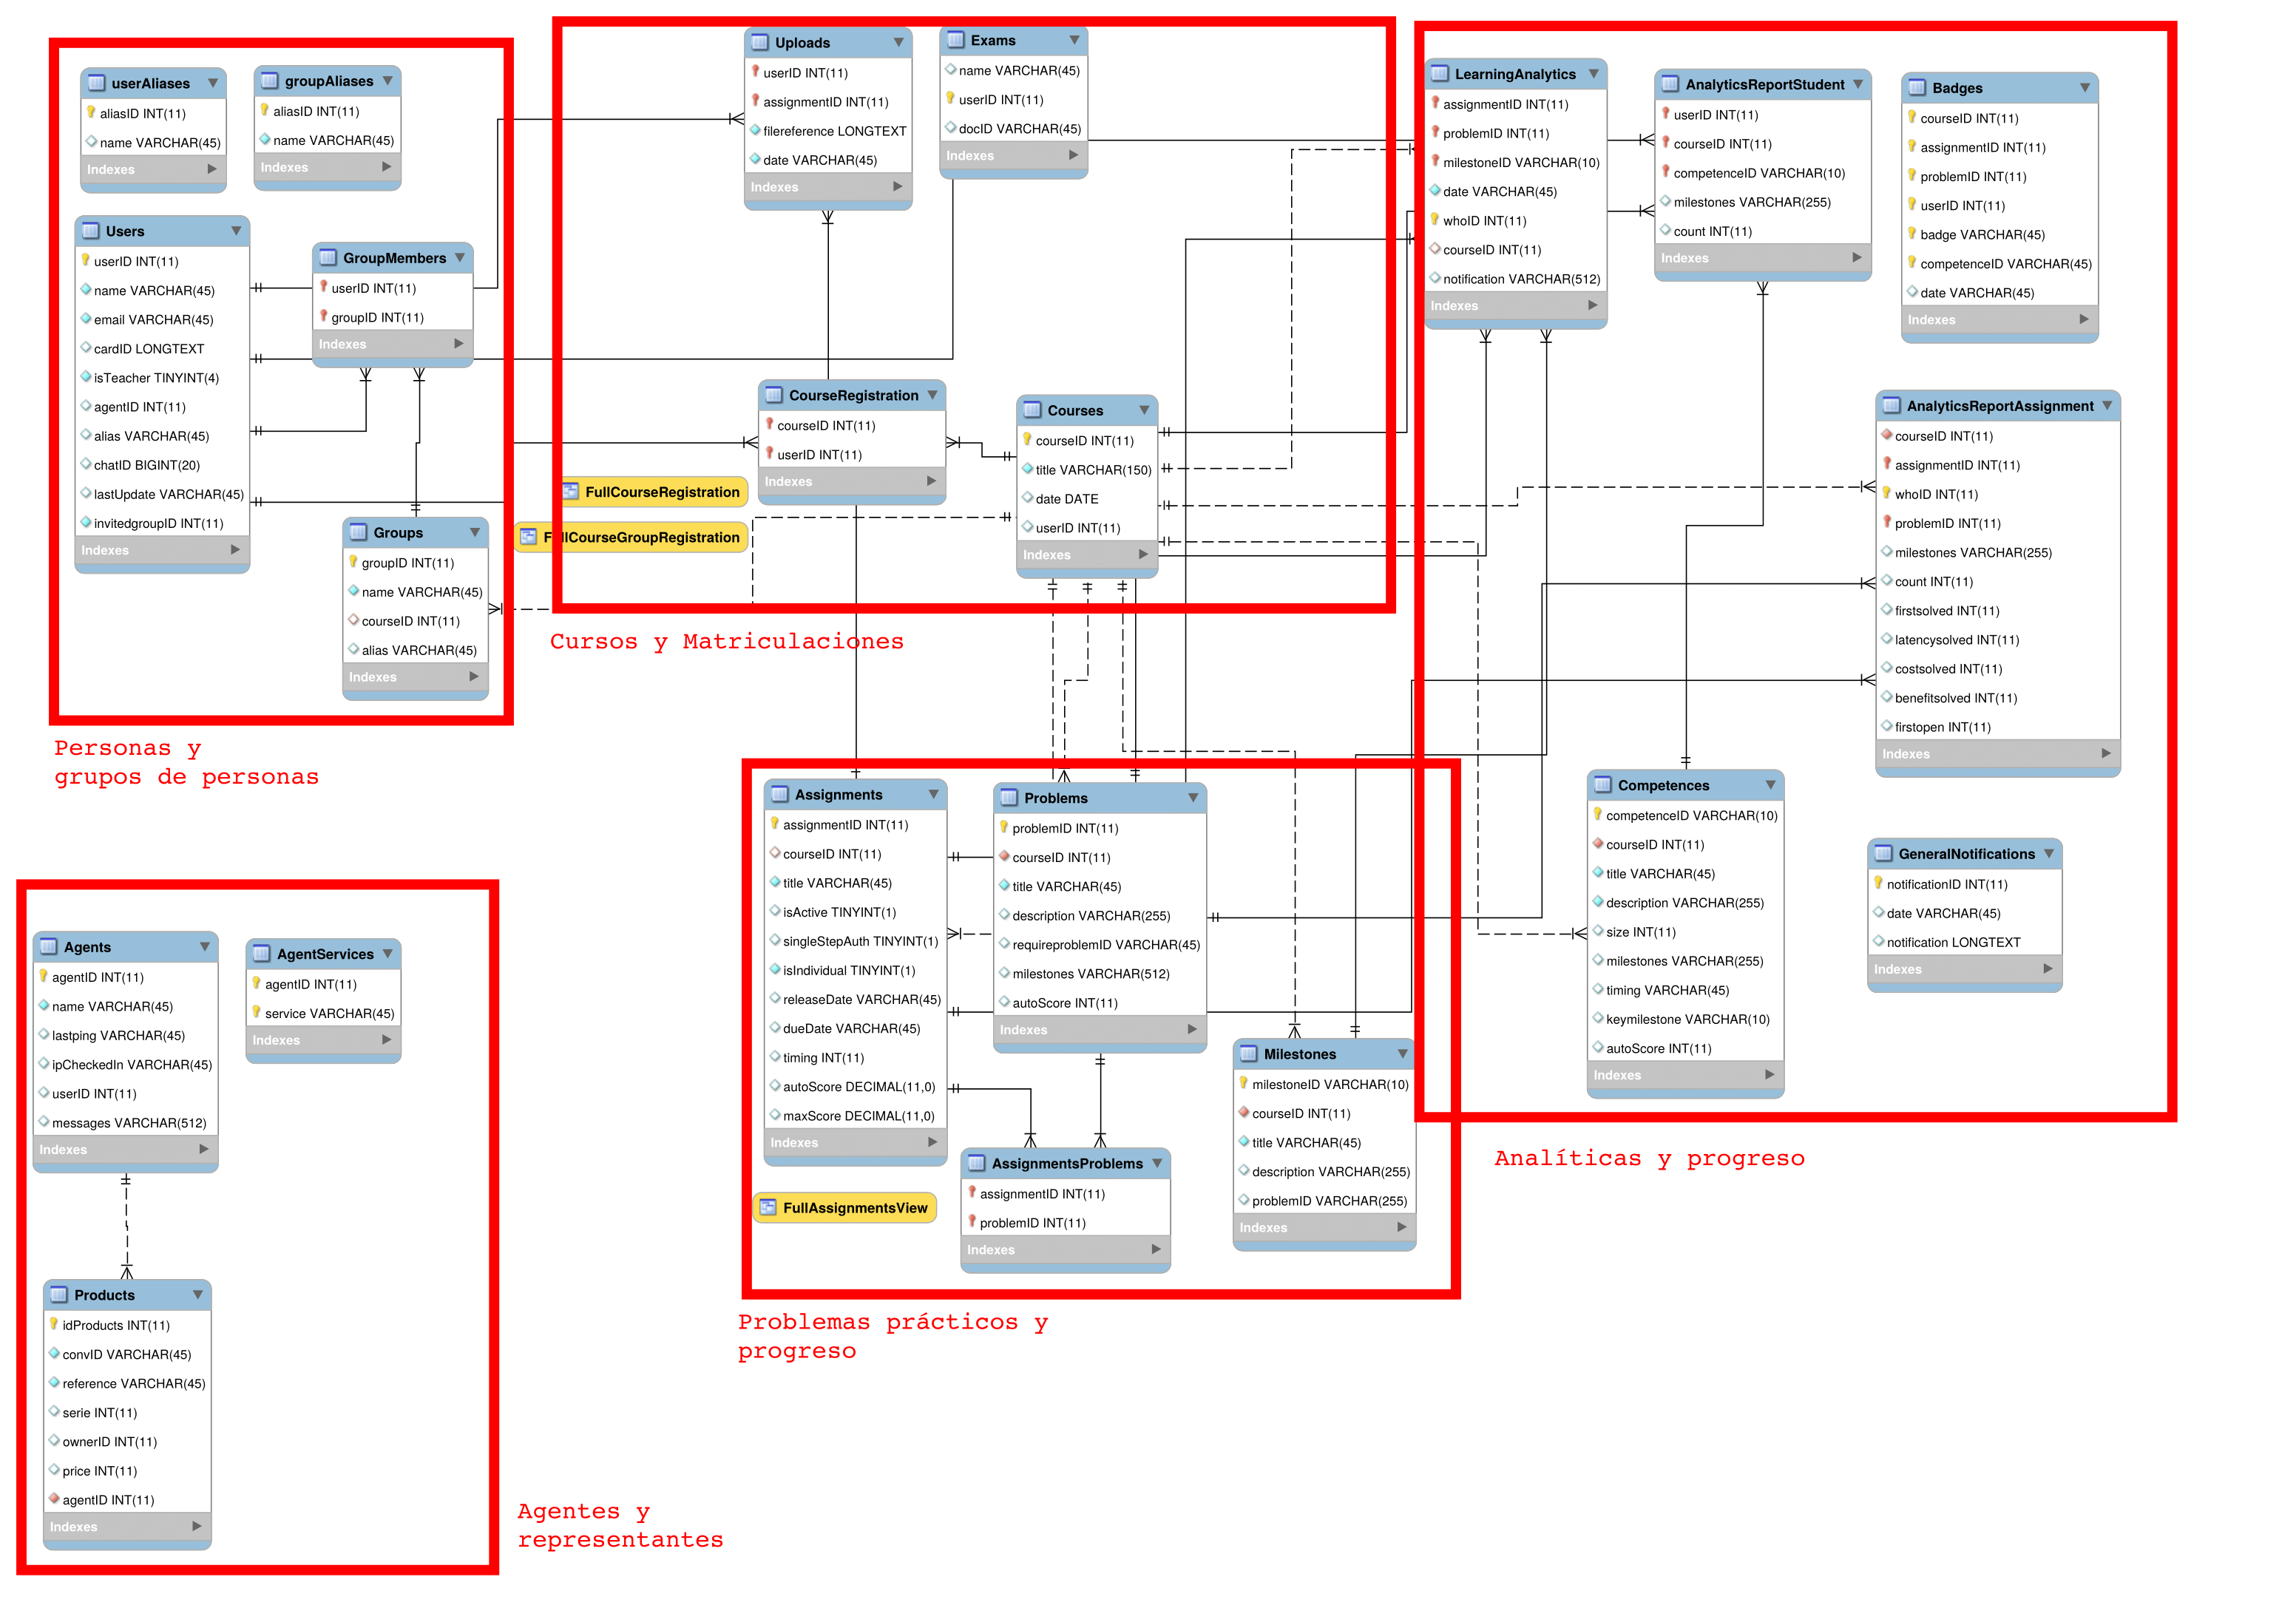
\includegraphics[width=1.35\textwidth]{logos/erbd.png}\\[1.4cm]
\caption{Diagrama entidad-relación de la base de datos del proyecto al inicio del mismo}
\label{img:erbd}
\end{figure}

\section{Bot de Telegram}

Todo lo relacionado con el comportamiento actual del bot de Telegram se gestiona a través de un servicio lanzado al mismo ecosistema de agentes de la asignatura y que se mantiene a la espera de recibir las comunicaciones de otros agentes o de los propios alumnos.\\

El funcionamiento de este bot, parte de enviar nuestra \textbf{cardID} como archivo al mismo bot. Éste hará las comprobaciones necesarias y verificará tu identidad para futuras comunicaciones con el mismo. Una vez verificada tu identidad, se establecerá una conexión con tu persona dentro de la asignatura y con tu chat único en Telegram. A través de ahí, se podrá hacer uso de los distintos comandos para obtener la retroalimentación correspondiente. Además, el bot nos informará de la ejecución de una práctica concreta: qué movimientos estamos haciendo, en qué estamos fallando, cuándo hemos completado una meta...
	
	\chapter{Planificación}

\section{Metodología utilizada}

Incluso desde el inicio de la asignatura Desarrollo Basado en Agentes, el profesor de dicha asignatura D. Luis Castillo Vidal nos exigió el uso de metodologías ágiles para el desarrollo de cada una de las prácticas, que se desarrollaban por grupos generalmente.\\

Para controlar todo el progreso de cada uno de los miembros, el profesor nos facilitó ciertas hojas de cálculo, una para cada grupo, donde cada grupo se encargaría de definir los siguientes elementos:

\begin{itemize}
	\item Cada una de las tareas que se van a llevar a cabo a lo largo de la práctica actual.
	\item Estimación de cuántas horas cada alumno se compromete a dedicar en la práctica actual.
	\item Estimación de cuántas horas cada tarea (o historia) puede ocupar. Es necesario que la suma de esta estimación coincida con la suma de la estimación de horas de cada alumno del grupo.
	\item Registrar las horas dedicadas a cada historia por parte de cada alumno.
	\item Definir, para cada práctica, un miembro del grupo que ejercerá como líder. Es quien debería de mantener las comunicaciones con el profesor.
\end{itemize}

De igual forma, para este proyecto se ha seguido una estrategia similar, que podría definir informalmente como \textit{pseudo-SCRUM}. En los primeros días de definición del proyecto, una vez estaban las bases consensuadas con mi tutor D. Luis Castillo Vidal, también hicimos una sesión de inicio de la metodología, en la que esencialmente llevamos a cabo algunas de las tareas mencionadas anteriormente.\\

Más concretamente, definimos la fecha de comienzo y fin del proyecto, y también definimos una serie de \textit{sprints}, con una cantidad fija de días cada uno tras los cuales organizaríamos una sesión de control para evaluar cómo iba avanzando el proyecto. Además, se consensuaron todas las historias a realizar durante todo el proyecto y se hizo la estimación general en horas.

\section{Temporización}

Antes de comentar en profundidad la temporización, es destacable comentar que inicialmente se realizó una fase de análisis en febrero, por la cual se estipuló dar comienzo al proyecto el día 3 de marzo del presente año y marcarlo como finalizado el día 15 de julio también del presente año, dividido en siete \textit{sprints} de 21 días cada uno a excepción del último. Debido a ciertos problemas, nos vimos obligados a posponer este proyecto y a realizar una nueva fase de replanificación en junio.\\

Durante la fase de análisis del proyecto, se llegó a un consenso con el tutor de establecer como fecha de comienzo el día 7 de junio de 2021 y fecha de finalización del mismo el 14 de septiembre del mismo año. Esta vez, se estipularon diez \textit{sprints} de diez días cada uno.\\

El proyecto se temporizó en 100 unidades de tiempo a completar, donde cada unidad de tiempo equivaldría entre tres y cuatro horas de trabajo real del alumno.\\

También se reestructuraron, en consenso con el tutor, las historias que previamente habíamos considerado para el proyecto en febrero para así ajustar de nuevo el tiempo que teníamos disponible y también teniendo en cuenta el trabajo previo que realicé anteriormente.\\

Surgieron así, 13 tareas o historias que deberían ser completadas a lo largo del periodo planificado anteriormente. En la tabla \ref{tab:historias}, se muestra un resumen de cada historia junto con el tiempo consensuado con el tutor.\\

En dicha tabla no obstante, aparecen 14 historias, y si además sumamos el tiempo estimado para cada una de estas historias, obtendríamos que el total de unidades de tiempo planificadas es de 112 en lugar de 100. Esto se debe a que en febrero, en la fase inicial de análisis, a pesar de que no se pudo seguir adelante con el proyecto, yo como estudiante llevé a cabo algunas tareas de investigación y comprensión que formaban parte de la planificación original, y que no se incluyeron de nuevo en la planificación ya que estaban completadas. Es por eso que se incluyeron de manera adicional indicando el número de horas que ya se había trabajado en el proyecto.

% Please add the following required packages to your document preamble:
% \usepackage{graphicx}
\begin{table}[]
\centering
\resizebox{\textwidth}{!}{%
\begin{tabular}{|l|l|c|}
\hline
\textbf{Historia}                                                                          & \textbf{Descripción}                                                                                                                                                                                                                                                                                                                                                                                                                                & \textbf{Tiempo Estimado} \\ \hline
Completar ciclo de simulador                                                               & \begin{tabular}[c]{@{}l@{}}Leer, interpretar y ejecutar archivos de registro completos. \\ Desde que se analiza cada línea del archivo, \\ hasta que se hace la comunicación con el agente de \\ Telegram.\end{tabular}                                                                                                                                                                                                                             & 7                        \\ \hline
Simular varios receptores                                                                  & \begin{tabular}[c]{@{}l@{}}Probar la recepción de mensajes de Telegram a \\ diferentes usuarios\end{tabular}                                                                                                                                                                                                                                                                                                                                        & 5                        \\ \hline
Procesar entradas de chat \#1                                                              & Identificación de cada usuario usando su cardID                                                                                                                                                                                                                                                                                                                                                                                                     & 5                        \\ \hline
Procesar entradas de chat \#2                                                              & \begin{tabular}[c]{@{}l@{}}Definir opciones de suscripción para notificaciones,\\ siendo capaz de definir:\\ - Recibir o no notificaciones\\ - Si se reciben notificaciones: recibir todas las \\ notificaciones, recibir solo las notificaciones\\ imprescindibles (mensajes de error)\\  o recibir notificaciones de tipo ACL\end{tabular}                                                                                                        & 12                       \\ \hline
Ofrecer progresos individuales                                                             & \begin{tabular}[c]{@{}l@{}}Perfil de progreso individual (o de grupo para aquellas \\ prácticas que sean en grupos)\end{tabular}                                                                                                                                                                                                                                                                                                                    & 7                        \\ \hline
Ofrecer progreso por problema                                                              & Perfil de progreso por un problema concreto                                                                                                                                                                                                                                                                                                                                                                                                         & 5                        \\ \hline
Ofrecer progreso por práctica                                                              & Perfil de progreso por una práctica concreta                                                                                                                                                                                                                                                                                                                                                                                                        & 7                        \\ \hline
Retroalimentaciones simples                                                                & - Fecha de entrega de una práctica concreta                                                                                                                                                                                                                                                                                                                                                                                                         & 6                        \\ \hline
\begin{tabular}[c]{@{}l@{}}Desplegar el sistema a un \\ entorno de producción\end{tabular} & \begin{tabular}[c]{@{}l@{}}Gestionar información en tiempo real, con conexión \\ directa a la base de datos y con agentes reales.\\ Verificar todas las historias previas.\end{tabular}                                                                                                                                                                                                                                                             & 15                       \\ \hline
Procesar entradas de chat \#3                                                              & \begin{tabular}[c]{@{}l@{}}Comprobar el estado de los agentes. Informar\\  al profesor a través de Telegram si uno de los \\ agentes no se encuentra disponible.\end{tabular}                                                                                                                                                                                                                                                                       & 5                        \\ \hline
Documentación                                                                              & Elaboración de la memoria                                                                                                                                                                                                                                                                                                                                                                                                                           & 16                       \\ \hline
Presentación                                                                               & Elaboración de la presentación para la defensa del proyecto                                                                                                                                                                                                                                                                                                                                                                                         & 10                       \\ \hline
Trabajo previo (desde febrero)                                                             & \begin{tabular}[c]{@{}l@{}}En resumen:\\ - Lectura de manuales de JADE\\ - Análisis y comprensión de proyectos relacionados con \\ \textit{behaviours} para entender mejor su funcionamiento\\ - Análisis y comprensión de la arquitectura LARVA\\ - Estudio de agentes y componentes concretos: ConfigFile, \\ Logger, ACLMessageQueue, ACLMSplitQueue,\\  Jerarquía de agentes...\\ - Estudio de la API de Telegram\end{tabular} & 12                       \\ \hline
\end{tabular}%
}
\caption{Backlog de historias estimadas para el proyecto. Cada unidad de tiempo corresponde a 3-4 horas de trabajo real del alumno.}
\label{tab:historias}
\end{table}

\section{Seguimiento del desarrollo}

El seguimiento de cada uno de los \textit{sprints} y de cada una de las tareas se realizó mediante una hoja de cálculo alojada en Google Drive, la cual fue puesta a punto y configurada por el tutor de este proyecto, adaptándola a las necesidades concretas del mismo.\\

La finalidad de esta hoja de cálculo es controlar el número de horas que se dedican a cada una de las historias, en cada uno de los diez \textit{sprints} que se estipularon. De esta forma y gracias a las configuraciones realizadas por el tutor, es posible ver de una forma muy visual el progreso tanto del proyecto a nivel general como del \textit{sprint} que se desee, como se muestra en la figura \ref{img:sprint3}.\\

\begin{figure}[h]
\centering
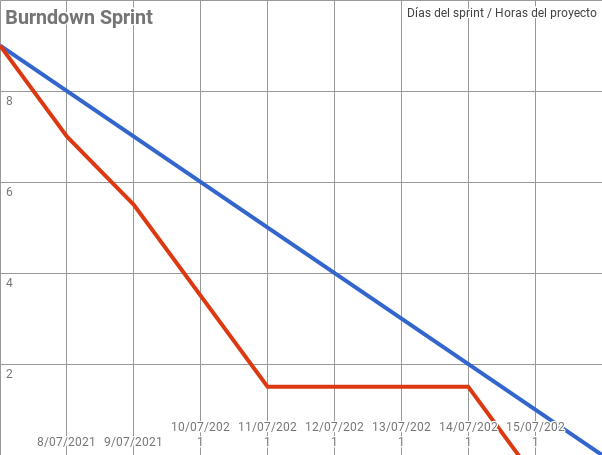
\includegraphics[width=0.9\textwidth]{logos/sprint4.png}\\[1.4cm]
\caption{Progreso del \textit{sprint} número 3. La línea azul representa el progreso ideal, mientras que la línea roja es el progreso real del estudiante durante ese \textit{sprint}.}
\label{img:sprint3}
\end{figure}

Como estudiante, me gustaría destacar que este procedimiento para llevar la cuenta de todas las horas dedicadas al proyecto resulta muy eficiente, ya que constantemente se obtiene retroalimentación real de cuánto va avanzando el proyecto, tanto a nivel general como a nivel concreto de historias.

\section{Diagrama de Gantt}

A continuación, en la figura \ref{img:gantt}, se presenta un diagrama de Gantt en el que se puede apreciar el trabajo realizado durante cada sprint en las distintas tareas previamente mencionadas.

\begin{figure}[h]
\centering
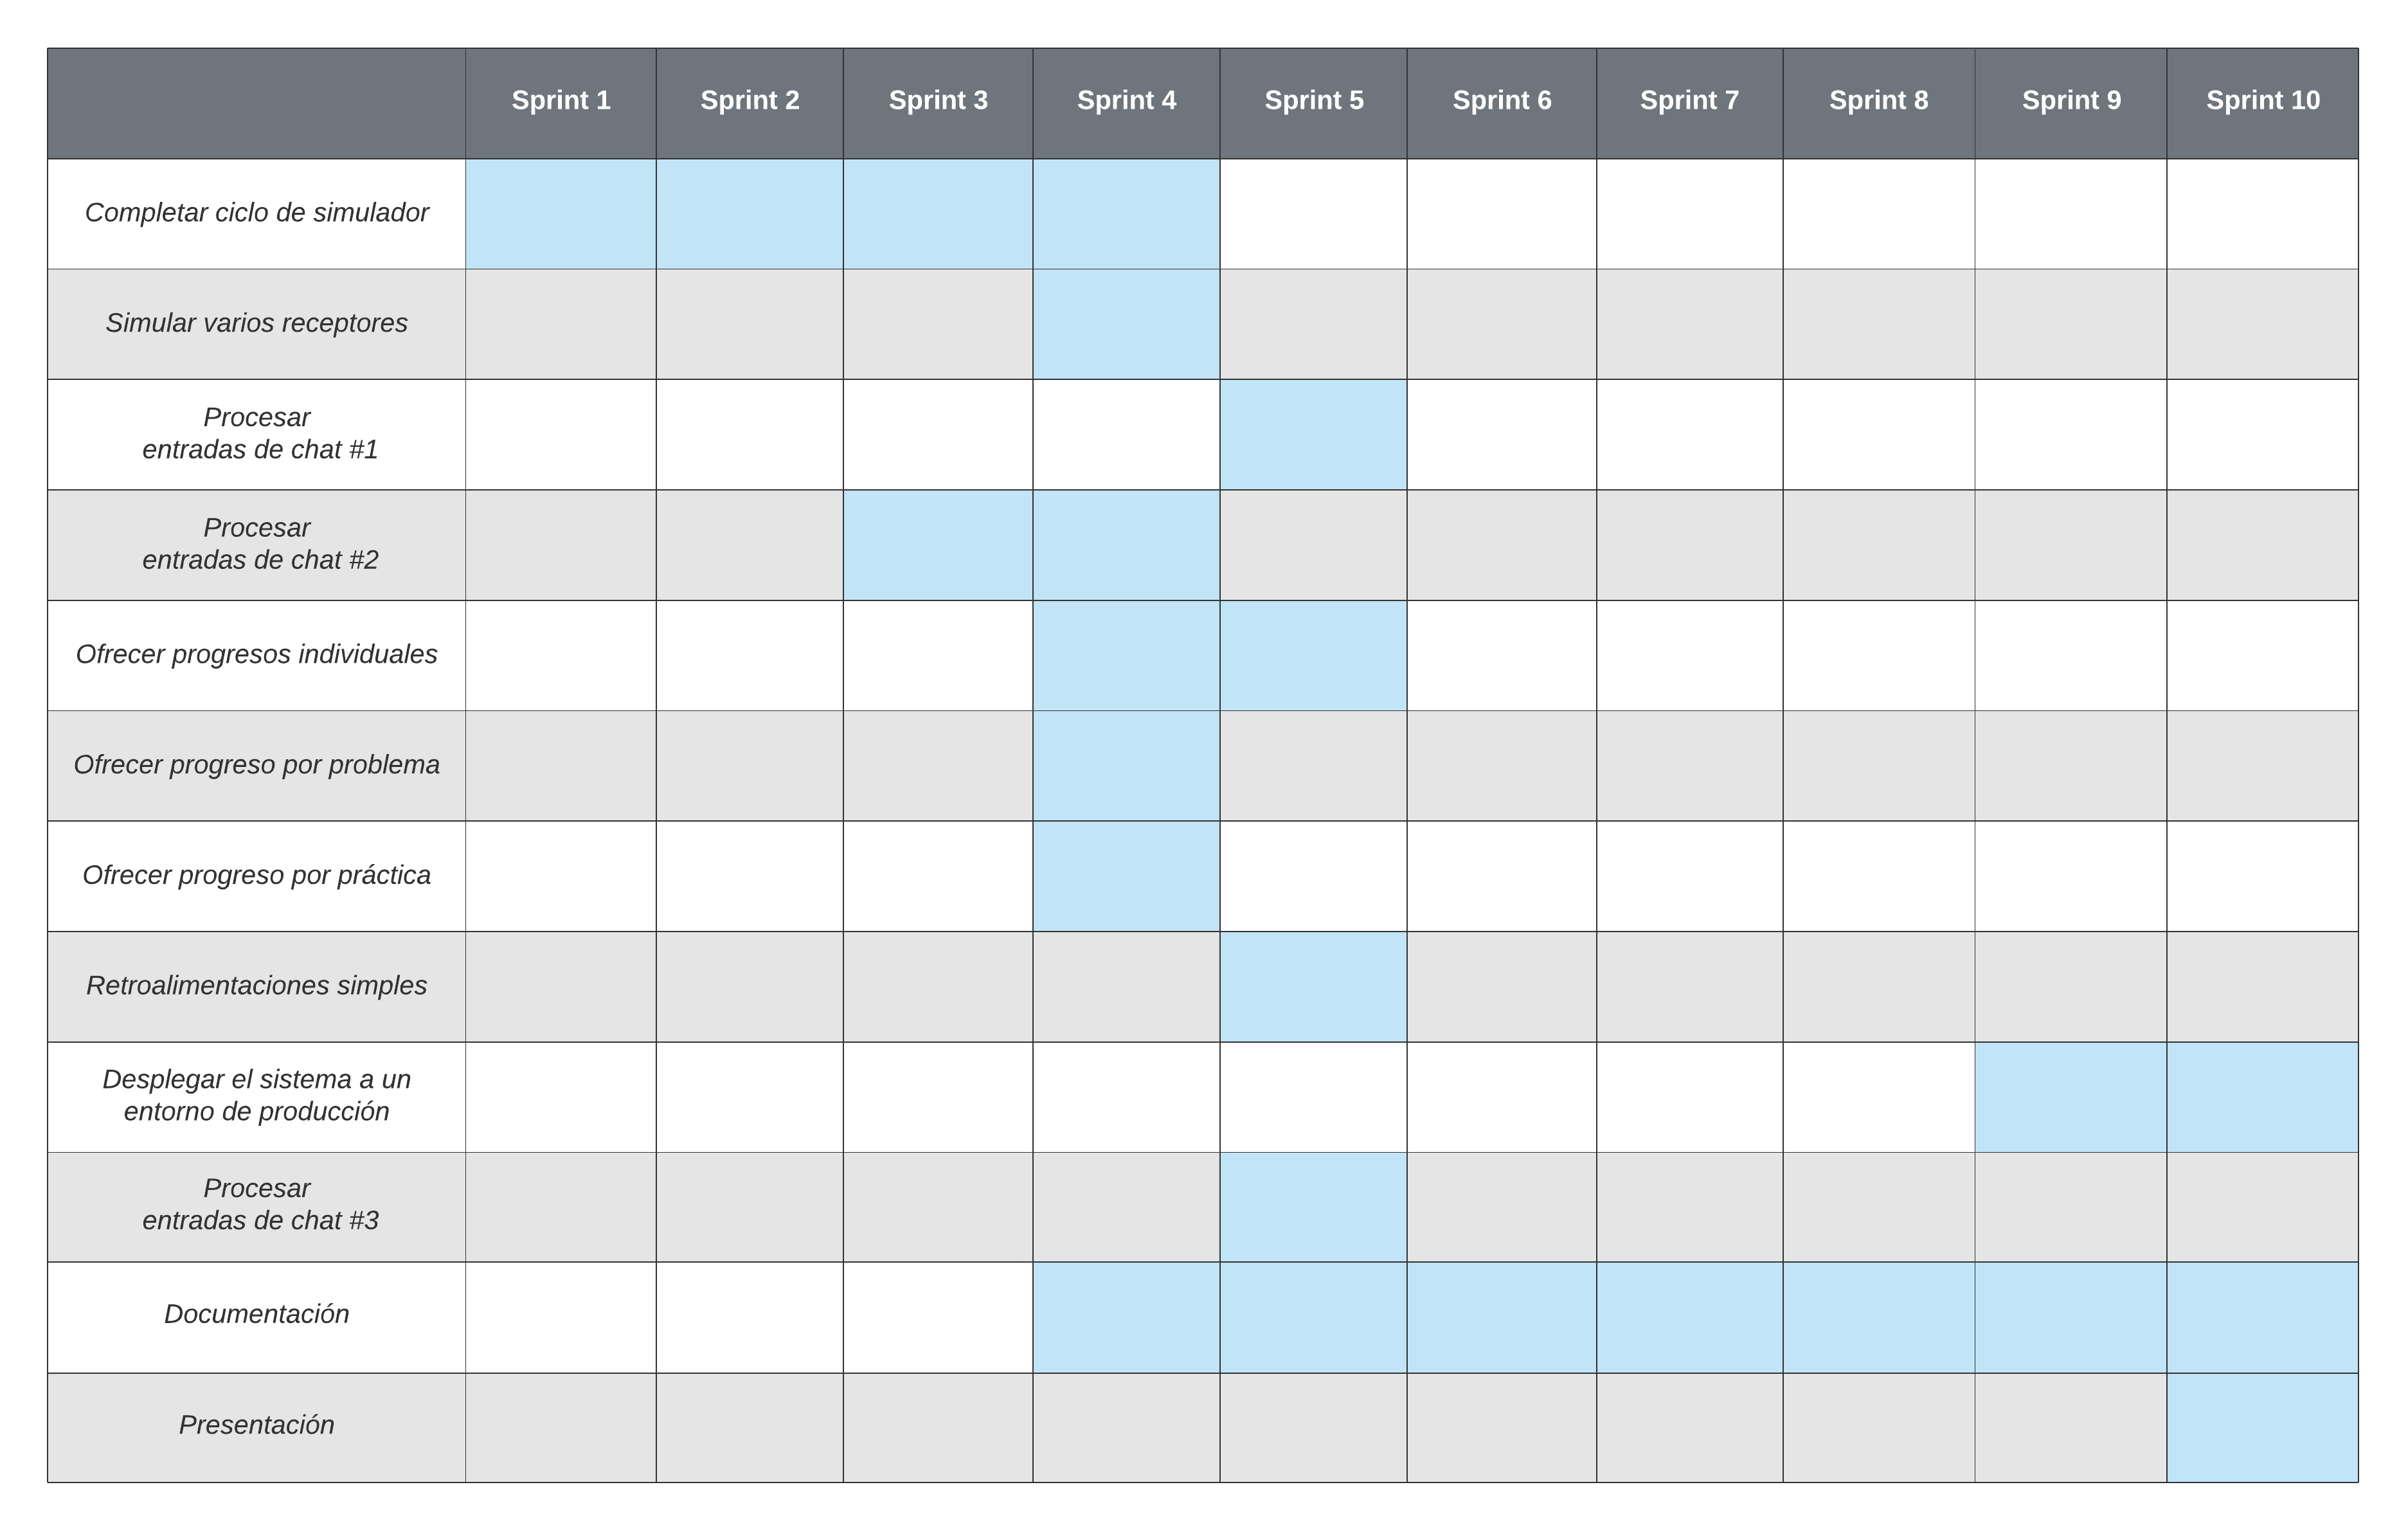
\includegraphics[width=1.1\textwidth]{logos/gantt.png}\\[1.4cm]
\caption{Diagrama de Gantt de la planificación}
\label{img:gantt}
\end{figure}

\section{Recursos}

\subsection{Recursos Humanos}

Los recursos humanos que han intervenido en la realización de este proyecto han sido, como autor del mismo, Francisco Domínguez Lorente y como tutor y supervisor del proyecto, D. Luis Castillo Vidal.

\subsection{Recursos Hardware}

Se han utilizado principalmente dos equipos durante el desarrollo del proyecto, ambos propiedad del autor del mismo, en este caso Francisco Domínguez Lorente:\\

\begin{itemize}
	\item Ordenador personal de sobremesa con procesador AMD Ryzen 5 3600 BOX, tarjeta gráfica Sapphire Radeon RX580 Nitro+, 16GB de memoria RAM y sistema operativo Ubuntu 20.04
	\item Dispositivo móvil Xiaomi Mi 9T Pro con la aplicación Telegram instalada
\end{itemize}

\subsection{Recursos Software}

Con respecto a los recursos a nivel de software que han sido usados en el proyecto, algunos ya han sido mencionados y otros se comentarán con más detalle en el siguiente capítulo. A saber, son:\\

\begin{itemize}
	\item Entorno de desarrollo NetBeans 12. Licencia libre.
	\item Librerías proporcionadas por el tutor del proyecto: LARVA, JADE, JDK
	\item Git y GitHub para el control de versiones
	\item Ubuntu 20.04 y Android 11 como sistemas operativos
	\item Telegram, en sus versiones para móvil y para ordenador
\end{itemize}

\subsection{Estimación de costos}

Con respecto a los recursos humanos, dentro del plan de estudios de la titulación, este propyecto tiene una carga lectiva de 12 créditos ECTS. Lo cual, sabiendo que cada crédito ECTS equivale a 25 horas, se puede traducir en aproximadamente 300 horas de trabajo.\\

Según la Universidad Europea \cite{universidad-europea-2021}, el salario de un ingeniero informático puede oscilar entre los 1.000 y 1.200 euros netos mensuales, por lo cual tomaré de referencia una cuantía de 8 euros netos por hora. Al haber sido estimado este proyecto 300 horas, el coste total de los recursos humanos será de 2.400 euros netos.\\

A continuación, con respecto a los recursos hardware, es necesario realizar ciertas estimaciones sobre la amortización de los dispositivos para saber cuánto coste han supuesto los mismos durante toda la duración del proyecto. Usaremos como referencia la tabla de coeficientes de amortización lineal proporcionada por la Agencia Tributaria \cite{amortizacion-agencia-tributaria}.\\

El primer dispositivo hardware, el ordenador personal, tuvo un coste final de 1000 euros. El periodo de amortización para sistemas informáticos es de 6 años, lo cual quiere decir que cada año se estima un coste de 166,67 euros del dispositivo. Al haberse desarrollado este proyecto durante los meses de febrero y septiembre \textit{(aproximadamente 7 meses)}, el coste estimado del dispositivo para el proyecto será de 97,25 euros.\\

De igual forma, el dispositivo móvil tuvo un coste final de 330 euros. Siguiendo las mismas indicaciones que en el párrafo anterior, el coste estimado del dispositivo para este proyecto habrá sido de 32 euros.\\

Los recursos software no han implicado costes adicionales, ya que todos ellos han sido obtenidos de manera gratuita siguiendo las indicaciones de las licencias de los mismos.\\

Así pues, se estima que el coste total del proyecto será de 2.529,25 euros sin tener en cuenta gastos adicionales como pueden ser la conexión a internet o el consumo de electricidad de los dispositivos, que pueden ser más complicados de calcular y de estimar.


	% Desarrollo bajo sprints: 
	% 	1. Permitir registros y login de usuarios
	% 	2. Desarrollo del sistema de incidencias
	% 	3. Desarrollo del sistema de denuncias administrativas y accidentes
	% 	4. Desarrollo del sistema de croquis
	%   5. Instalación de la aplicación de manera automática
	\chapter{Implementación}

\section{Configuración del entorno en NetBeans 12}

El proceso de configuración del entorno en la plataforma de desarrollo NetBeans 12, la cual también usamos durante el desarrollo de la asignatura Desarrollo Basado en Agentes, fue cuanto menos tedioso. Todo el conglomerado de proyectos que posibilitan la ejecución de LATEN es necesario configurarlo, idealmente, a la vez y de manera uniforme.\\

Los diferentes proyetos fueron proporcionados por el tutor del proyecto de manera gradual, para de igual forma intentar acoplarlos al nuevo proyecto que se creó, perteneciente al propio agente LATEN. Esto en un primer momento ocasionó problemas de dependencias, tanto de proyectos como de archivos Java \textit{(con terminación .jar)}, incluso de otros paquetes de apoyo.\\

No obstante, tras unas horas de trabajo conjunto con el tutor, se pudo configurar de manera total el proyecto LATEN y el resto de proyectos auxiliares.\\

Los proyectos de NetBeans de los que depende LATEN de una manera u otra, se listan a continuación:

\begin{itemize}
	\item BaseTelegram
	\item CoreLARVAAdminObjects
	\item CoreLARVAAgents
	\item CoreLARVAObjects
	\item CoreLARVAMoreObjects
	\item PTelegram
\end{itemize}

Adicionalmente, se requieren también los siguientes archivos con terminación \textit{.jar}:

\begin{itemize}
	\item Conector Java-MySQL, versión 8.0.25
	\item JADE
	\item La librería de utilidades Commons IO
\end{itemize}

Es importante mencionar también que se requiere de la versión 11 de JDK \textit{(\textbf{J}ava \textbf{D}evelopment \textbf{K}it)} para el correcto funcionamiento de todos los proyectos.\\

Una vez se tienen todos los proyectos correctamente importados, y las librerías debidamente incorporadas, se puede proceder con el resto de configuraciones necesarias antes de poder empezar con la implementación de nuestro agente.

\section{Configuración de la base de datos}

Con respecto a la configuración de la base de datos, el profesor de la asignatura me proporcionó un script SQL para poder tener una copia local de la base de datos tal y como se había usado para la asignatura. En dicha copia de la base de datos, se eliminaron aquellos datos de carácter sensible de otros alumnos que no influirían posteriormente en el propio proyecto, como por ejemplo el correo electrónico institucional de la Universidad de Granada o el número de identificación del chat personal de Telegram de cada alumno.\\

Para la gestión de la base de datos es buena práctica usar un cliente, ya sea web o con aplicación nativa, ya que permite una mejor visualización de toda la estructura de la base de datos, así como de los propios datos que alberga. Es evidente que también se puede usar la terminal de, en mi caso, el sistema operativo Ubuntu 20.04, para llevar a cabo todas las labores de gestión de la base de datos.\\

En mi caso, por preferencias personales, decidí instalar el gestor \textbf{phpMyAdmin}, el cual es una interfaz gráfica de usuario disponible a través de web, accediendo desde la dirección \textit{http://localhost/phpmyadmin}.\\

Para la instalación de dicho cliente desde la terminal de Ubuntu 20.04, se deben seguir unos pasos concretos. En primer lugar, se debe ejecutar el comando

\begin{lstlisting}
    sudo apt update
\end{lstlisting}

para actualizar la lista de paquetes disponibles y sus versiones. A continuación, el comando para proceder a la instalación del paquete de phpMyAdmin, así como de sus dependencias es el siguiente:

\begin{lstlisting}
    sudo apt install phpmyadmin php-mbstring php-gettext
\end{lstlisting}

Este comando, al ejecutarlo, nos ofrecerá una interfaz gráfica para especificar ciertos parámetros de configuración para el cliente. Entre ellos, deberemos establecer las contraseñas del usuario administrador de la base de datos, así como de la propia aplicación MySQL. Además, deberemos de seleccionar en qué servidor web queremos que se ejecute phpMyAdmin: \textit{apache2} o \textit{lighttpd}. Escogí \textit{apache2} por estar más familiarizado con el mismo.\\

Una vez completado el proceso de instalación mediante la terminal, ya podremos acceder a la interfaz gráfica a través del enlace anteriormente mencionado: \textit{http://localhost/phpmyadmin}.\\

El siguiente paso, será importar el script SQL que facilitó el tutor de la asignatura. Desde la interfaz gráfica, primeramente deberemos crear la base de datos en la que posteriormente importaremos dicho script. A la base de datos, le otorgué el nombre \textbf{LATEN}. Se puede crear una base de datos de manera muy sencilla como se muestra en la figura \ref{img:menubd1}. Basta con introducir el nombre de la base de datos que queremos crear y posteriormente pulsar sobre el botón \textbf{Crear}.

\begin{figure}[h]
\centering
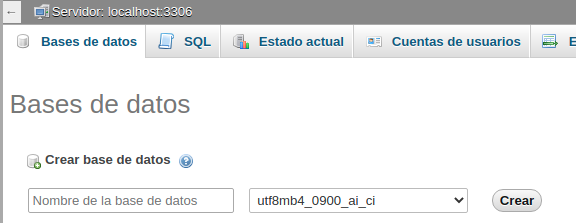
\includegraphics[width=0.9\textwidth]{logos/menubd1.png}\\[1.4cm]
\caption{Pestaña de creación de base de datos en phpMyAdmin}
\label{img:menubd1}
\end{figure}

Una vez creada la base de datos, navegaremos hacia ella a través de la interfaz gráfica y pulsaremos sobre el botón \textbf{Importar} del menú superior de phpMyAdmin. En esta ventana, podremos importar fácilmente el archivo con extensión \textit{.sql} aportado por el tutor de la asignatura, como se muestra en la figura \ref{img:menubd2}. Una vez cargado el script, presionaremos sobre el botón \textbf{Continuar} situado al pie de dicha página, y acto seguido tendremos disponible nuestra base de datos, con todas las tablas y con todos los datos correspondientes.

\begin{figure}[h]
\centering
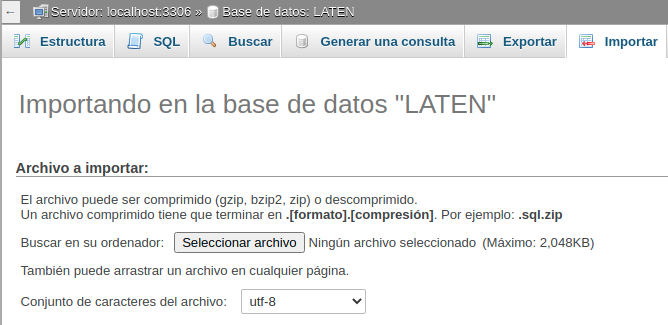
\includegraphics[width=0.9\textwidth]{logos/menubd2.png}\\[1.4cm]
\caption{Pestaña de importación en phpMyAdmin}
\label{img:menubd2}
\end{figure}


\section{Configuración y entorno de JADE}

Como se explicó en la sección \ref{sec:jade}, JADE es un framework que actuará de middleware entre nuestro sistema de agentes.\\

Su configuración es bastante sencilla. En la ya mencionada asignatura, se nos proporcionó un fichero comprimido que contiene todo lo necesario para la instalación de JADE. Con la siguiente secuencia de comandos, instalaremos de manera muy sencilla el paquete:

\begin{lstlisting}
    unzip dba-jade-kit.zip
    cd bin
    sudo ./install.sh
\end{lstlisting}

Una vez instalado, podemos ejecutar el servicio de JADE haciendo uso del siguiente comando:

\begin{lstlisting}
    sudo ./doJade.sh start
\end{lstlisting}

y de igual forma, cambiando el argumento, para detener el servicio:

\begin{lstlisting}
    sudo ./doJade.sh stop
\end{lstlisting}

Estas herramientas que acabamos de instalar también gozan de una interfaz gráfica desde la que observar todos los agentes que se encuentran disponibles en la plataforma además de las comunicaciones que se realizan entre ellos. Para ejecutar dicha interfaz gráfica, usaremos el siguiente comando:

\begin{lstlisting}
    sudo ./doJadeGUI.sh 
\end{lstlisting}

El cual, tras unos instantes nos mostrará una pantalla como la que se muestra en la figura \ref{img:jade1}.

\begin{figure}[h]
\centering
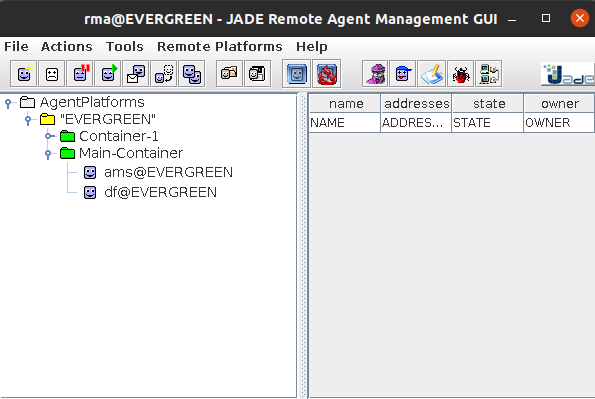
\includegraphics[width=0.9\textwidth]{logos/jade1.png}\\[1.4cm]
\caption{Interfaz gráfica de JADE}
\label{img:jade1}
\end{figure}

\section{Configuración del agente}

Para que nuestro agente se integre de manera correcta en la red con el resto de agentes que ya habitan en ella, es necesario especificar ciertos parámetros de configuración que posteriormente serán leídos por las clases correspondientes que lanzan dicho agente a la plataforma JADE. Estos parámetros de configuración se establecerán en formato JSON, dentro de una carpeta llamada \textit{config} del mismo proyecto de nuestro agente LATEN.\\

Dichos parámetros de configuración son los que se muestran a continuación:

\begin{lstlisting}
    {
        "name": "LATEN",
        "version": "1.0",
        "silent": false,
        "log": true,
        "system": true,
        "showbehaviour": false,
        "singlebehaviour": true,
        "boot": "jade",
        "jadeconnection": {
            "host": "localhost",
            "port": 1099
        },
        "dbconnection": {
            "host": "localhost",
            "port": 3306,
            "database": "LATEN",
            "user": "username",
            "password": "password"
        }
    }
\end{lstlisting}

A destacar de este archivo de configuración, podemos ver el elemento \textbf{singlebehaviour}, el cual tiene como valor asignado \textit{true}, lo cual indica que dicho agente tiene un solo comportamiento y por tanto no es necesario establecer configuraciones adicionales a la hora de lanzar dicho agente, como por ejemplo sería establecer un sistema de colas múltiple para la recepción de mensajes ACL.\\

Otros elementos como \textbf{silent}, \textbf{log} o \textbf{system}, tienen como propósito informar al desarrollador sobre los distintos acontecimientos durante la ejecución de dicho agente. Se pueden configurar a \textbf{true} o \textbf{false} para ajustar la cantidad de información que queremos recibir de la ejecución.\\

Adicionalmente, tenemos un elemento de configuración de la conexión de JADE llamado \textbf{jadeconnection}, en el que podemos especificar el \textbf{host} y el \textbf{puerto \textit{(port)}} a través de los cuales se puede establecer una conexión con JADE.\\

Por último, tenemos el elemento \textbf{dbconnection} que posee toda la configuración necesaria para establecer conexión con la base de datos previamente configurada.

\section{Implementación}

\subsection{Agente LATEN}

El agente LATEN en un inicio se planificó como el agente encargado de interactuar con el resto de los agentes de la red, haciendo de puente entre aquellos agentes destinados a la resolución de las prácticas, como los ya mencionados \textbf{WorldManagers} y entre el propio bot de Telegram.

\subsubsection{Clase principal}

En todo el ecosistema ya mencionado, los agentes se lanzan a la plataforma esencialmente de la misma forma, con quizás algunos cambios. Se puede apreciar en el siguiente fragmento de código, en el que explicaré brevemente en qué consiste cada línea.

\begin{lstlisting}
    static ConsoleBoot _app;

    public static void main(String[] args) {
        _app = new ConsoleBoot("LATEN", args);
        _app.selectConnection();
        _app.launchAgent(LATEN.class);
        _app.shutDown();
    }
\end{lstlisting}

Para comenzar, creamos un objeto de clase de la clase \textbf{ConsoleBoot}, la cual es una clase creada por el profesor de la asignatura para ejecutar aplicaciones JADE con todo lo necesario para que los agentes se puedan ejecutar \textbf{(y ser cerrados)} de manera segura ya sea en nuestra máquina local o en remoto.\\

El siguiente método \textbf{selectConnection()}, selecciona la conexión que hayamos definido en nuestro archivo de configuración JSON, ya sea nuestra máquina local o una máquina remota, como podría ser el propio servidor de la asignatura para realizar las propias prácticas.\\

\textbf{launchAgent()} básicamente lanza al agente a la plataforma y el método \textbf{shutDown()} cerrará el agente junto con los contenedores creados cuando el método \textbf{plainExecute()} de la clase \textbf{LATEN} termine de ejecutarse y por tanto haya finalizado el trabajo del agente.

\subsubsection{El método plainExecute()}

Este es el método principal de la clase \textbf{LATEN}. Es el que se ejecutará durante toda la vida útil del agente. El propósito actual de dicho agente es el de leer, interpretar y actuar sobre los distintos registros de las sesiones prácticas de la asignatura. Al comienzo de este proyecto, el tutor me facilitó los registros reales de las prácticas del grupo de prácticas al que yo pertenecía durante la asignatura, los cuales usé para poder implementar y probar esta funcionalidad.\\

Al lanzar el agente LATEN a la plataforma, para proceder a la lectura e interpretación de los registros, se siguen los siguientes pasos:\\

\begin{enumerate}
    \item Identificar el grupo al que pertenece dicho registro
    \item Identificar los miembros de dicho grupo
    \item Obtener los ajustes de noticaciones específicos de cada usuario del grupo
    \item Analizar cada línea y enviar los mensajes correspondientes al agente de Telegram para que éste informe a los miembros correspondientes
\end{enumerate}

Los tres primeros puntos de la lista anterior se pueden observar, de manera breve en el siguiente fragmento de código:

\begin{lstlisting}
    // Identify which group does this communication belong to
    this.group = this.identifyGroup(myReader.nextLine());
    
    // Verify which members do we have to send the message to
    // First, obtain the groupID
    JsonObject groupID = _dataBase.queryJsonDB("SELECT groupID FROM LATEN.Groups WHERE alias='" + this.group + "'").getRowByIndex(0);
    
    // Members belonging to that group
    JsonArray usersID = _dataBase.queryJsonDB("SELECT userID FROM GroupMembers WHERE cardID IS NOT NULL AND groupID=" + groupID.get("groupID")).getAllRows();
    
    for(int i = 0; i < usersID.size(); i++) {
        this.groupMembers.add(usersID.get(i).asObject());
    }
    
    // Adds the notifications settings for each user
    for(JsonObject groupMember : this.groupMembers) {
        JsonObject usersNotifications = 
                _dataBase.queryJsonDB("SELECT notificationSettings FROM Users WHERE userID=" + groupMember.get("userID")).getRowByIndex(0);
        
        groupMember.add("notificationSettings", usersNotifications.get("notificationSettings"));
    }
\end{lstlisting}

Como se puede observar, se realizan varias consultas a la base de datos y estos datos se van almacenando en ciertas variables de la clase para su posterior uso.\\

Con respecto al último punto, al comienzo del método se declaran las siguientes variables, que sirven para abrir y leer el archivo correspondiente de las sesiones:

\begin{lstlisting}
    File ficheroSesiones = new File(sessionFile);
    Scanner myReader = new Scanner(ficheroSesiones);
\end{lstlisting}

De tal forma, una vez se hayan hecho todas las consultas necesarias a la base de datos y almacenado los datos correspondientes, podremos iterar sobre cada línea del registro con un bucle y así analizar y actuar sobre cada línea:

\begin{lstlisting}
    while(myReader.hasNextLine()) {
        String linea = myReader.nextLine();
        
        JsonObject jsonLine = Json.parse(linea).asObject();
        String info;
        
        if (linea.contains("acl_receive_REGULAR") && linea.contains("\"command\":\"login\"")) {
            // This is a notification marked as ALL
            String newConvIDs = this.buildNotificationString("ALL");                
            
            sendMessage("PTelegram", ACLMessage.AGREE, "REGULAR", Emojis.ENVELOPE + " Sending login request...", newConvIDs);
            
        } else if (linea.contains("acl_send_REGULAR") && linea.contains("Login request from")) { [...]
\end{lstlisting}

\subsubsection{Métodos auxiliares}

En el método \textbf{plainExecute()} se han podido observar otras funciones auxiliares que se programaron para modularizar lo máximo posible el agente y hacerlo así más legible, y sobre todo más mantenible de cara a un futuro. A continuación se comentan las más relevantes:\\

La primera que procedo a comentar es quizás la más destacable y la más usada, ya que en cada condición diferente del bucle principal del método \textbf{plainExecute()} se usa. Es la función encargada de mandar un mensaje a un determinado agente de la plataforma. Recibe ciertos parámetros como el nombre del agente, la performativa a enviar, o el contenido, como se puede observar a continuación:\\

\begin{lstlisting}
    /**
     * Sends a message
     * @param receiver Message's receiver
     * @param performative The performative to use
     * @param protocol Message's protocol
     * @param content Message's content
     * @param conversationID The conversation ID to send the message to
     */
    protected void sendMessage(String receiver, int performative, String protocol, String content, String conversationID) {
        ACLMessage out = new ACLMessage();
        out.setSender(this.getAID());
        out.addReceiver(new AID(receiver, AID.ISLOCALNAME));
        out.setPerformative(performative);
        out.setProtocol(protocol);
        out.setContent(content);

        if(conversationID != "") {
            out.setConversationId(conversationID);
        }

        this.send(out);
    }
\end{lstlisting}

Como observamos en la función anterior, es necesario proveer de un \textit{conversationID}, que es esencialmente una cadena de caracteres, que puede estar separada por espacios, en la que se indica cada uno de los chats a los que se les debe entregar cada mensaje. Así pues, en la siguiente función lo que se hace es constuir esa cadena de caracteres en base a las preferencias de notificaciones de cada usuario:\\

\begin{lstlisting}
    /**
     * Returns an updated list of conversation IDs to send the notifications
     * @param notification rank
     * @return String containing the conversation IDs
     */
    protected String buildNotificationString(String notification) {
        String convIDs = "";
        
        for (JsonObject groupMember : this.groupMembers) {
            for (String type : notification.trim().split(" ")) {
                if (groupMember.get("notificationSettings")
                .toString().replaceAll("\"", "").equals(type)) {
                    convIDs = convIDs + " " + groupMember.get("userID").toString();
                }
            }
        }
        
        return convIDs;
    }
\end{lstlisting}

De tal modo, en la siguiente línea se especifica que se debe enviar ese mensaje concreto, a aquellos usuarios que tengan las preferencias de notificaciones en \textit{''ALL''}:\\

\begin{lstlisting}
    // This is a notification marked as ALL
    String newConvIDs = this.buildNotificationString("ALL");
\end{lstlisting}

Como ya se ha comentado en otras ocasiones, debido a falta de tiempo y otros diversos problemas, no se ha podido proceder al lanzamiento de este agente a la plataforma con el resto de agentes de la asignatura. Se comentarán más detalles en la sección de trabajos futuros.

\subsection{Agente PTelegram \textit{(Public Telegram)}}

El agente correspondiente al proyecto PTelegram, denominado de igual forma en la plataforma de agentes, es aquel que se encargará esencialmente de procesar todas las actualizaciones que lleguen tanto de Telegram como a través de mensajes provenientes de otros agentes en la red. Este proyecto parte del proyecto inicialmente desarrollado por el profesor, llamado \textbf{PublicTelegram}, y el motivo por el que crear uno idéntico a ese y renombrarlo a \textbf{PTelegram} fue esencialmente por facilidad a la hora del desarrollo, tal y como sugirió el tutor del proyecto.\\

Este agente hereda del agente \textbf{BaseTelegram}, que proporciona funcionalidad abstracta para su posterior implementación. El motivo de tener esta clase padre, es que en la asignatura existen dos tipos de bots de Telegram: el bot destinado a los alumnos \textit{(PublicTelegram)} y el bot destinado al profesor \textit{(PrivateTelegram)}.

\subsubsection{Clase principal}

Como podemos observar en el siguiente fragmento de código, la manera de inicializar el agente perteneciente a \textit{PTelegram} es prácticamente idéntica a la del agente \textit{LATEN}. La única diferencia, obviamente, es el nombre que se le pasa como parámetro al crear el objeto de la clase \textbf{ConsoleBoot}:\\

\begin{lstlisting}
    public static void main(String[] args) {
        ConsoleBoot app = new ConsoleBoot("AgentTelegram", args);
        app.selectConnection();
        app.launchAgent(PublicTelegram.class);
        app.shutDown();
    }
\end{lstlisting}

\subsubsection{El método plainExecute()}

Como se ha mencionado anteriormente, la clase \textbf{PTelegram} hereda de \textbf{BaseTelegram}, y por lo tanto esta clase hija no tiene un método \textit{plainExecute()} definido, si no que usará por defecto el de la clase padre.\\

Es importante diferenciar entre dos tipos de actualizaciones que le llegaran al agente. En primer lugar, tenemos las actualizaciones que llegan evidentemente desde cada chat de Telegram. Esto es, cuando un usuario utiliza cualquiera de los comandos operativos en el mismo. Además, tenemos las actualizaciones provenientes del resto de agentes de la red y más concretamente para este proyecto, aquellos mensajes que son enviados desde nuestro agente \textbf{LATEN} hacia el agente \textbf{PTelegram} para proceder a la difusión de mensajes en los chats correspondientes.\\

Por tanto, la misión del método \textit{plainExecute()}, que recordemos que se ejecuta \textit{''indefinidamente''}, será la de comprobar periódicamente si existen actualizaciones de cualquiera de los dos tipos mencionados y procesarlas como sea necesario:\\

\begin{lstlisting}
    @Override
    public final void plainExecute() {
        Update u; // Cola de mensajes de Telegram (Telegramchat)
        ACLMessage iu; // Cola de mensajes de LARVA blockingReceive()
    
        // Process one single update for every queue, to do a kind of leveled answer to all inbound requirements
        for (long cid : telegramQueue.getAllChatIDActive()) {
            u = telegramQueue.popUpdateChatID(cid);
            processTelegramUpdate(cid, u);
        }
        
        // Internal updates
        this.processACLMUpdates();
        if (this.internalUpdates.size() > 0) {
            iu = this.internalUpdates.get(0);
            this.internalUpdates.remove(0);
            processInternalUpdate(iu);
        }
        
        // Wait for a little while
        if (telegramQueue.isAllEmpty() && this.internalUpdates.isEmpty()) {
            doBlock(500);
        }
    }
\end{lstlisting}

Los dos método que se llaman en este método, \textit{processTelegramUpdate} y \textit{processInternalUpdate} son métodos abstractos de la clase \textbf{BaseTelegram} que deberán ser implementados ya sea en \textbf{PTelegram} o en \textbf{PrivateTelegram}.\\

Para comenzar, el método \textit{processTelegramUpdate} implementado en \textbf{PTelegram}, una vez recibe una actualización de un chat de Telegram, verifica que está haciendo uso de uno de los comandos establecidos y ejecuta la función correspondiente, como se puede observar en el siguiente fragmento de código \textit{(incompleto y adaptado a este documento)}:\\

\begin{lstlisting}
    @Override
    protected void processTelegramUpdate(long cid, Update u) {
        if (!isDebug || cid == this.LCastilloCID) {
            TelegramChat tc = this.telegramQueue.getChatData(cid);
            File cardfile;
            if (u.getMessage().hasText()) {
                String line = u.getMessage().getText(), parameters[] = line.split(" ");
                switch (parameters[0]) {
                    case "/help":
                        this.sendTelegram(cid, help(cid));
                        break;
                        
                    case "/notificationstatus":
                        doCheckNotificationsStatus(cid);
                        break;
                        
                    case "/myprogress":
                        doMyProgress(cid);
                        break;
                        
                    default:
                        this.sendTelegram(cid, hello);
        [...]
\end{lstlisting}

Por último, el método \textit{processInternalUpdate} actúa de manera similar. Tras unas comprobaciones iniciales, procede a comprobar qué performativa recibe del mensaje correspondiente y así realizar las accioens necesarias \textit{(fragmento de código incompleto y adaptado a este documento)}:\\

\begin{lstlisting}
    @Override
    protected void processInternalUpdate(ACLMessage msg) {
        ArrayList<Long> usersinvolved = new ArrayList();
        String what, convid = "";
        JsonObject jsreport;

        try {
            [...]
            switch (msg.getPerformative()) {
                case ACLMessage.REQUEST:
                    [...]
                    break;
                case ACLMessage.INFORM:
                    [...]
                    break;
                case ACLMessage.AGREE:
                    [...]
                    break;
            }
            
        [...]
\end{lstlisting}

\subsubsection{Métodos auxiliares}

Con respecto al resto de métodos auxiliares, en concreto para el método \textit{processTelegramUpdate}, se implementan en la propia clase \textbf{BaseTelegram} y se usa uno distinto para cada comando recibido a través de Telegram. Los más complejos requieren de algunas consultas a la base de datos.\\

Por poner un ejemplo, ya que algunos además de consultas a la base de datos requieren de algunos cálculos y comprobaciones adicionales, a continuación se muestra el método \textbf{doSetNotifications()}, que se llama cuando desde Telegram se recibe el comando \textit{/notifications <option>}. Desde la clase \textbf{PTelegram} se comprueba que los parámetros son correctos, y en tal caso, se llama al método \textbf{doSetNotifications()} que actualiza en la base de datos las preferencias de notificaciones del usuario de dicho chat.\\

Una vez hechas las consultas, se envía el mensaje correspondiente al chat del usuario. Un ejemplo del funcionamiento se puede visualizar en la figura \ref{img:exampletelegram}.

\begin{lstlisting}
    protected void doSetNotifications(long cid, String type) {
        TelegramChat tc = this.telegramQueue.getChatData(cid);
        
        try {
            _dataBase.updateDB("UPDATE Users SET notificationSettings='" + type + "' WHERE userID='" + tc.getUserID() + "'");
            this.sendTelegram(cid, Emojis.INFO + " Notifications set to " + type);
        } catch (Exception ex) {
            Exception("", ex);
            this.sendTelegram(cid, Emojis.WARNING + "I could not perform this task due to an internal error. Please try later");
        }
    }
\end{lstlisting}

\begin{figure}[h]
\centering
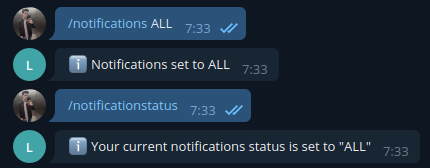
\includegraphics[width=0.9\textwidth]{logos/exampletelegram.png}\\[1.4cm]
\caption{Ejemplo del funcionamiento de los comandos \textit{/notifications <option>} y \textit{/notificationstatus} en el bot LATEN de Telegram}
\label{img:exampletelegram}
\end{figure}

Para una referencia completa de los comandos disponibles a través del bot y sus descripciones, véase la tabla \ref{tab:botcommands}.

\begin{table}[]
\centering
\resizebox{\textwidth}{!}{%
\begin{tabular}{|l|l|}
\hline
\textbf{Comando}    & \textbf{Descripción}                                                                                                                                                                                                                                                                                                  \\ \hline
/help               & Show the information of the commands                                                                                                                                                                                                                                                                                  \\ \hline
/link               & \begin{tabular}[c]{@{}l@{}}Bind this chat to the previously\\ uploaded identity (cardID)\end{tabular}                                                                                                                                                                                                                 \\ \hline
/whoami             & Checks the last stored identity                                                                                                                                                                                                                                                                                       \\ \hline
/notifications      & \begin{tabular}[c]{@{}l@{}}Establish the level of notifications\\ that you want to receive:\\ \\ ALL: Receive all notification messages\\ MIN: Receive only the critical\\ messages (errors and goal\\ achievements)\\ ACL: Receive only ACL updates\\ NONE: You won' receive\\ any notifications at all\end{tabular} \\ \hline
/notificationstatus & \begin{tabular}[c]{@{}l@{}}Check your current level of \\ notifications\end{tabular}                                                                                                                                                                                                                                  \\ \hline
/myprogress         & \begin{tabular}[c]{@{}l@{}}Outputs your current progress for\\ the whole subject\end{tabular}                                                                                                                                                                                                                         \\ \hline
/problemprogress    & \begin{tabular}[c]{@{}l@{}}Outputs your current progress for\\ a specific problem of an\\ assignment\end{tabular}                                                                                                                                                                                                     \\ \hline
/assignmentprogress & \begin{tabular}[c]{@{}l@{}}Outputs your current progress for all\\ the problems of the specified\\ assignment\end{tabular}                                                                                                                                                                                            \\ \hline
\end{tabular}%
}
\caption{Comandos disponibles en el bot de Telegram}
\label{tab:botcommands}
\end{table}

\subsection{Resto de clases y utilidades}

Además de los proyectos mencionados \textit{(LATEN, PTelegram y BaseTelegram)}, estos se valen de otros proyectos adicionales que han sido desarrollados por el profesor de la asignatura y que simplemente me gustaría comentar para contextualizar este proyecto, a pesar de que no han sido modificados en el ámbito de este proyecto.\\

En la siguiente lista se muestran algunas de las utilidades que considero más importantes:

\begin{itemize}
	\item Paquete \textbf{AdminKeys \textit{(en el proyecto CoreLARVAAdminObjects)}}: Implementa ciertas utilidades para la encriptación \textit{(y desencriptación)} de las ya mencionadas cardIDs
	\item Paquete \textbf{Database \textit{(en el proyecto CoreLARVAAdminObjects)}}: Todas las herramientas para poder hacer consultas a la base de datos
	\item Paquete \textbf{ControlPanel \textit{(en el proyecto CoreLARVAAgents)}}: Proporciona a los estudiantes a tener un panel de control visual para el desarrollo de las prácticas
	\item Paquete \textbf{Map2D \textit{(en el proyecto CoreLARVAMoreObjects)}}: Es el que visualmente, junto con el paquete \textbf{ControlPanel}, hace que se visualicen correctamente los mapas de las prácticas de la asignatura
\end{itemize}

Son más las utilidades que se proporcionan y que demuestran que ha sido un trabajo laborioso, largo y cuidado por parte del profesor de la asignatura.

\section{Entorno de producción. Agentes LATEN y PTelegram en acción.}

Quizás una de las partes más importantes de este proyecto es la de integrar ambos agentes en el ecosistema de agentes disponible para las prácticas de la asignatura. Esta es una tarea que requiere de manera imprescindible la presencia del tutor de este proyecto y profesor de la asignatura Desarrollo Basado en Agentes, D. Luis Castillo Vidal. El motivo es simple, solo él tiene acceso al servidor \textit{isg2.ugr.es}, el cual a través del puerto \textbf{1099} aloja la plataforma de JADE y las comunicaciones entre agentes para las prácticas de la asignatura.\\

Para realizar esto, uno de los días planificados del proyecto se realizó una tutoría entre ambas partes que duró aproximadamente dos horas y media, en la cual se pusieron en marcha todos los mecanismos necesarios para poder ejecutar un agente \textit{(ya sea de un grupo de alumnos o del profesor)} capaz de resolver uno de los mapas pertenecientes a las prácticas. Se reactivó y comprobó toda la infraestructura previa de la asignatura y se hicieron pequeñas adaptaciones para que los agentes \textbf{LATEN} y \textbf{PTelegram} se pudiesen ejecutar en conjunto en la red de agentes. Por ejemplo, y como se ha ejemplificado en el párrafo anterior, es necesario cambiar los datos de acceso tanto a JADE como a la base de datos de los archivos de configuración de ambos agentes, tal y como se muestra a continuación:\\

\begin{lstlisting}
    [...]
    "jadeconnection": {
        "host": "isg2.ugr.es",
        "port": 1099
    },
    "dbconnection": {
        "host": "isg2.ugr.es",
        "port": 3306,
        "database": "Agents",
        "user": "##",
        "password": "##"
    }
\end{lstlisting}

Es evidente que en dicha base de datos, la original tal y como se quedó tras la finalización de la asignatura necesitaba los cambios \textit{(que no fueron muchos)} para poder adaptarse a todo el comportamiento de los agentes.\\

Una vez puesta en marcha toda la infraestructura y estando disponible para que agentes externos interactúen con ella, es necesario seguir los siguientes pasos para comprobar el correcto funcionamiento de ambos agentes:\\

\begin{itemize}
	\item Ejecutar el proyecto \textbf{PTelegram} contra el servidor previamente mencionado, para ofrecer su disponibilidad de enviar mensajes a Telegram a aquellos usuarios que sea necesario
	\item Ejecutar el proyecto \textbf{LATEN} contra el servidor, estando así disponible a recibir las comunicaciones del agente \textbf{WorldManager} para poder procesarlas y enviar los mensajes \textit{(ACL)} necesarios a \textbf{PTelegram} 
	\item Ejecutar un agente programado por el profesor o por un grupo de alumnos que resuelva \textit{(o que lo intente)} un mapa concreto de una de las prácticas disponibles en la asignatura
\end{itemize}

El agente resolutor del mapa comenzará a hacer su trabajo tal y como ha sido programado. Las acciones que vaya realizando durante su ejecución serán comunicadas a los agentes que sean necesarios de la red, entre ellos, el \textbf{WorldManager} que replicará los mensajes que le devuelva al agente resolutor también a \textbf{LATEN}. \textbf{LATEN} procesará los mensajes conforme los reciba, y enviará los mensajes necesarios a \textbf{PTelegram}, quien se encargará de también hacer ciertas operaciones y procesos para así servir a los usuarios correspondientes los mensajes a través de Telegram.\\

Además, como \textbf{PTelegram} está activo y disponible, los usuarios también pueden hacer uso de las funcionalidades ya comentadas del propio bot. Estas serán procesadas únicamente por \textbf{PTelegram}, que hará las comprobaciones necesarias y devolverá a los chats de Telegram los mensajes requeridos por los usuarios.\\

En la figura \ref{img:ejecucion1}, se aprecia una ejecución en tiempo real de los agentes \textbf{LATEN} y \textbf{PTelegram} contra el servidor de la asignatura de Desarrollo Basasdo en Agentes. A la derecha, podemos observar la aplicación Telegram que recibe los mensajes procesados a través de \textbf{LATEN}. A la izquierda y en el centro de la imagen, observamos las interfaces gráficas de un agente que se está encargando de resolver un mapa de una práctica concreta, real, de dicha asignatura. Dicho agente también se está ejecutando contra el mismo servidor, por tanto los resultados obtenidos a la derecha, en la conversación con \textbf{LATEN}, son mensajes reales recibidos en tiempo real conforme el agente resolutor ha ido completando objetivos.

\begin{figure}[h]
\centering
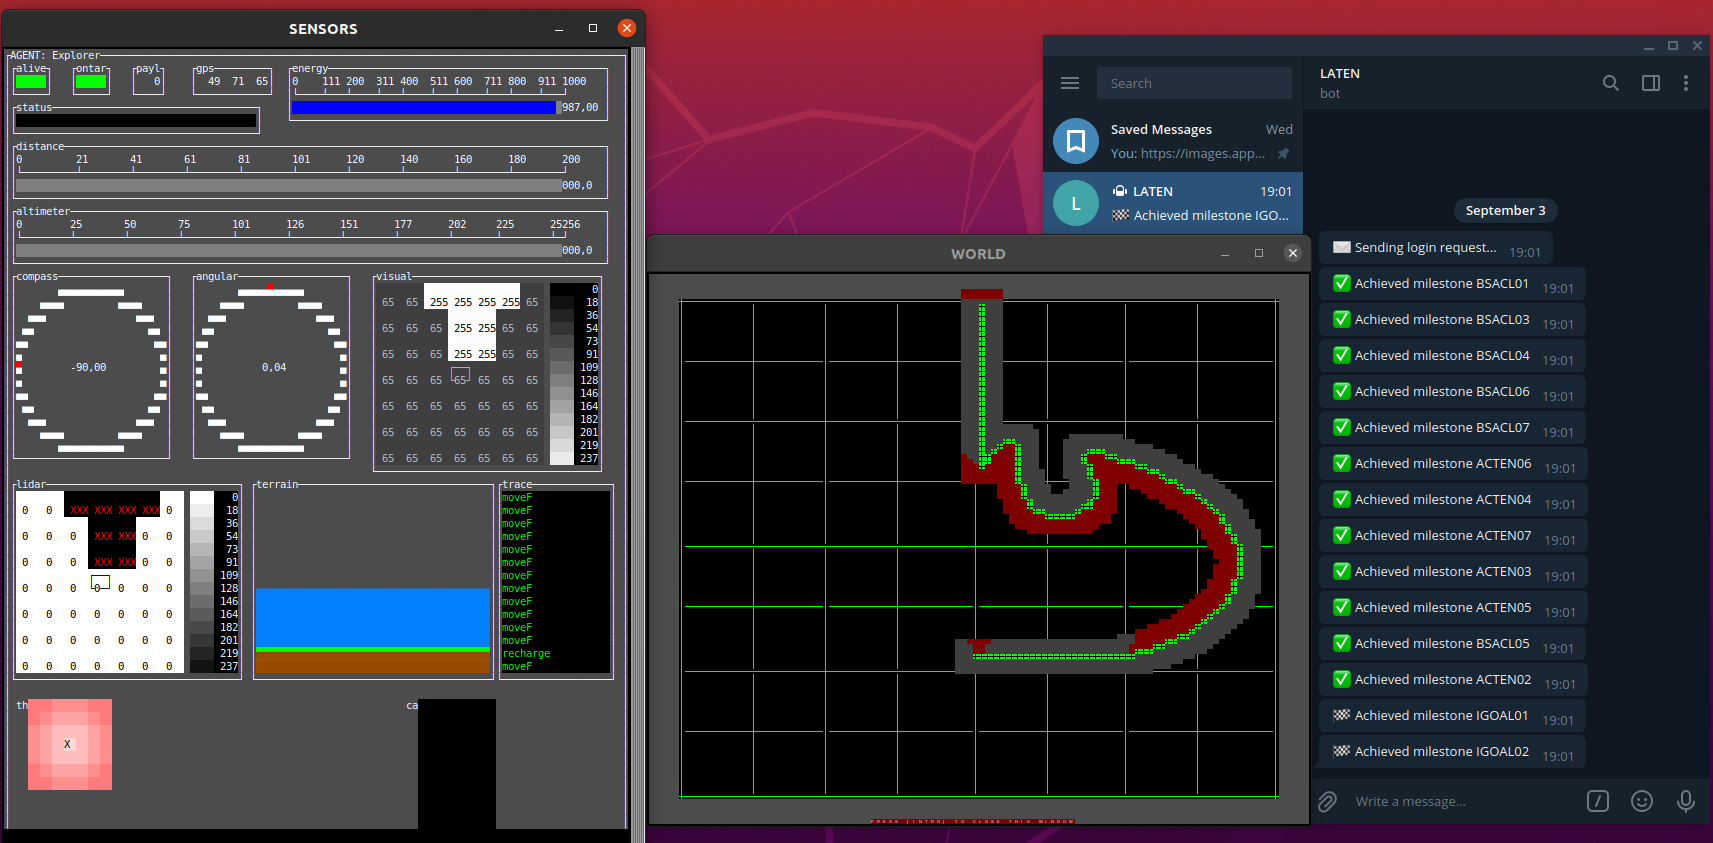
\includegraphics[width=1.1\textwidth]{logos/ejecucion1.png}\\[1.4cm]
\caption{Ejemplo de ejecución en tiempo real de LATEN, PTelegram y un agente resolutor de un mapa concreto}
\label{img:ejecucion1}
\end{figure}

\section{Diagrama de la aplicación}

A continuación, en la figura \ref{img:diagramaaplicacion} se muestra un diagrama simplificado y reducido de la aplicación en cuestión. A la izquierda del mismo se muestran los distintos agentes resolutores de las prácticas comunicándose con el \textbf{WorldManager}, quien replica las comunicaciones a \textbf{LATEN} que a su vez se comunica con \textbf{PTelegram}. En la parte superior se muestran las distintas utilidades que ya estaban presentes con anterioridad, explicadas en secciones anteriores de este proyecto y de las que heredan o importan el resto de agentes.

\begin{figure}[h]
\centering
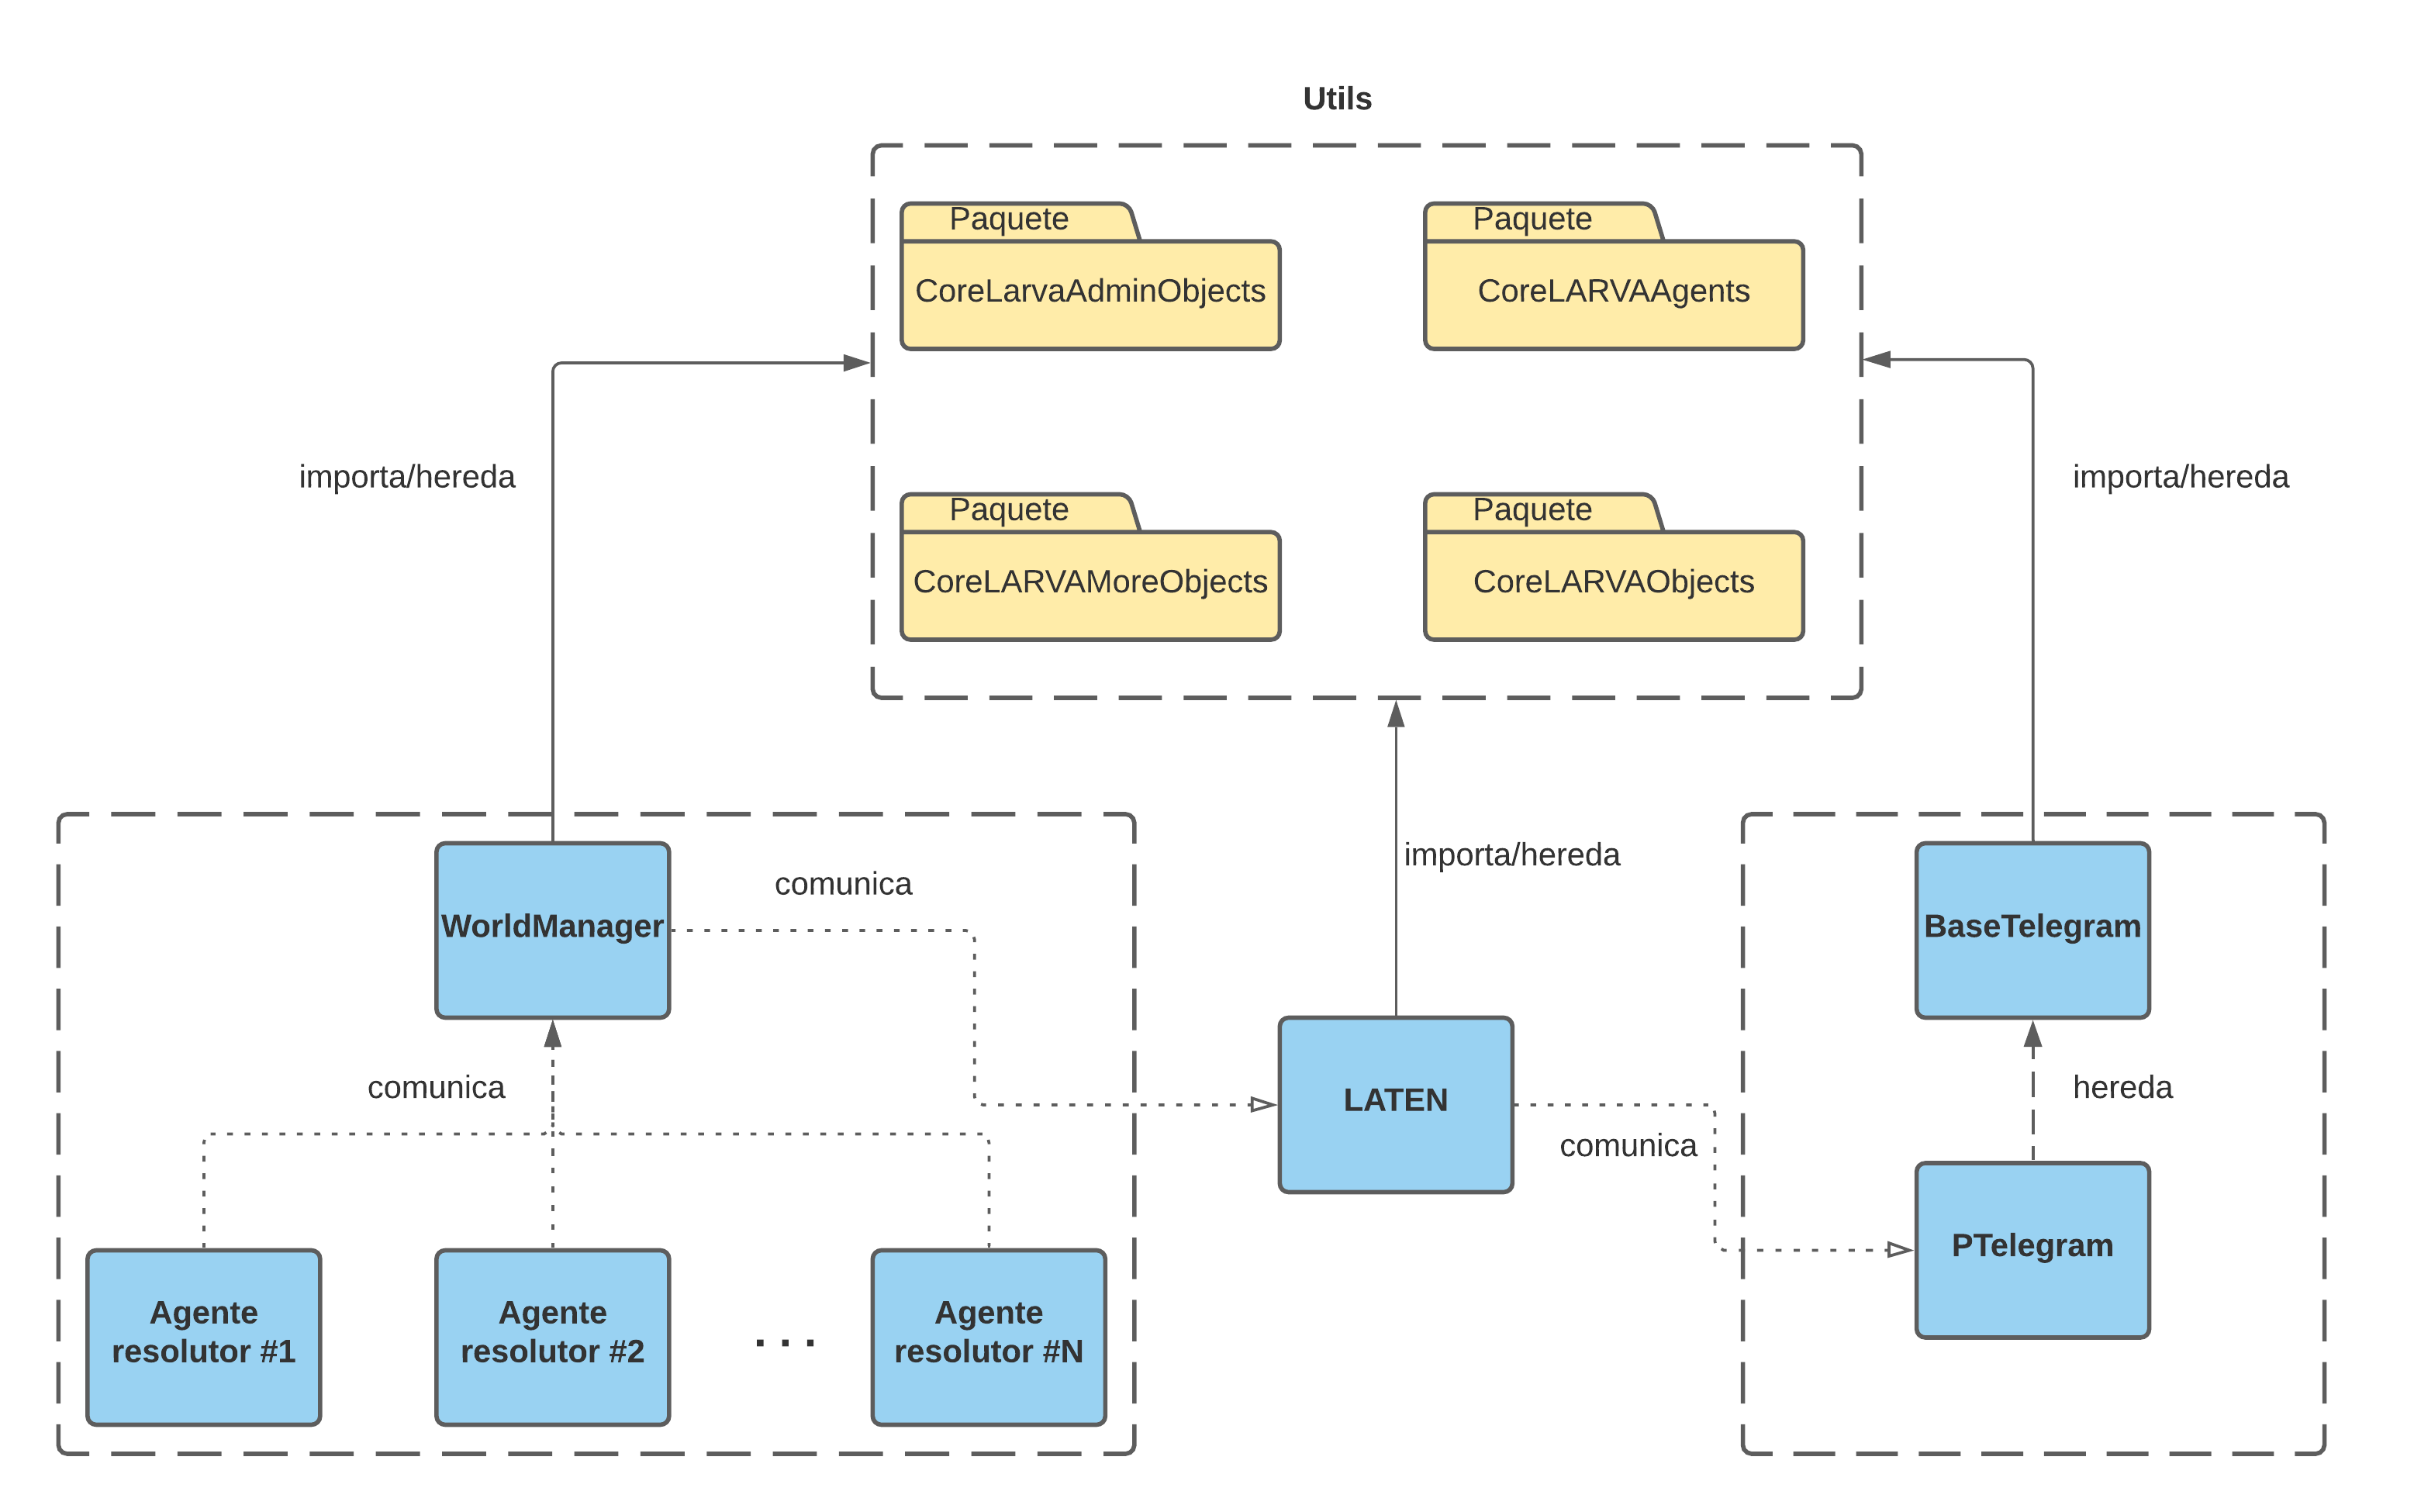
\includegraphics[width=1.1\textwidth]{logos/diagramaaplicacion.png}\\[1.4cm]
\caption{Diagrama simplificado de la aplicación}
\label{img:diagramaaplicacion}
\end{figure}

\section{Ejemplo de comunicación entre agentes}

Una herramienta para visualizar lo que está pasando por detrás y que nos servirá de ayuda para contextualizar las imágenes previamente dispuestas en el documento es un diagrama de secuencia. En la figura \ref{img:secuencia}, se muestra un diagrama de secuencia sencillo con el comportamiento esperado de la red de agentes que interactúan directamente, a través de \textbf{PTelegram} con el propio usuario en su chat de Telegram.

\begin{figure}[h]
\centering
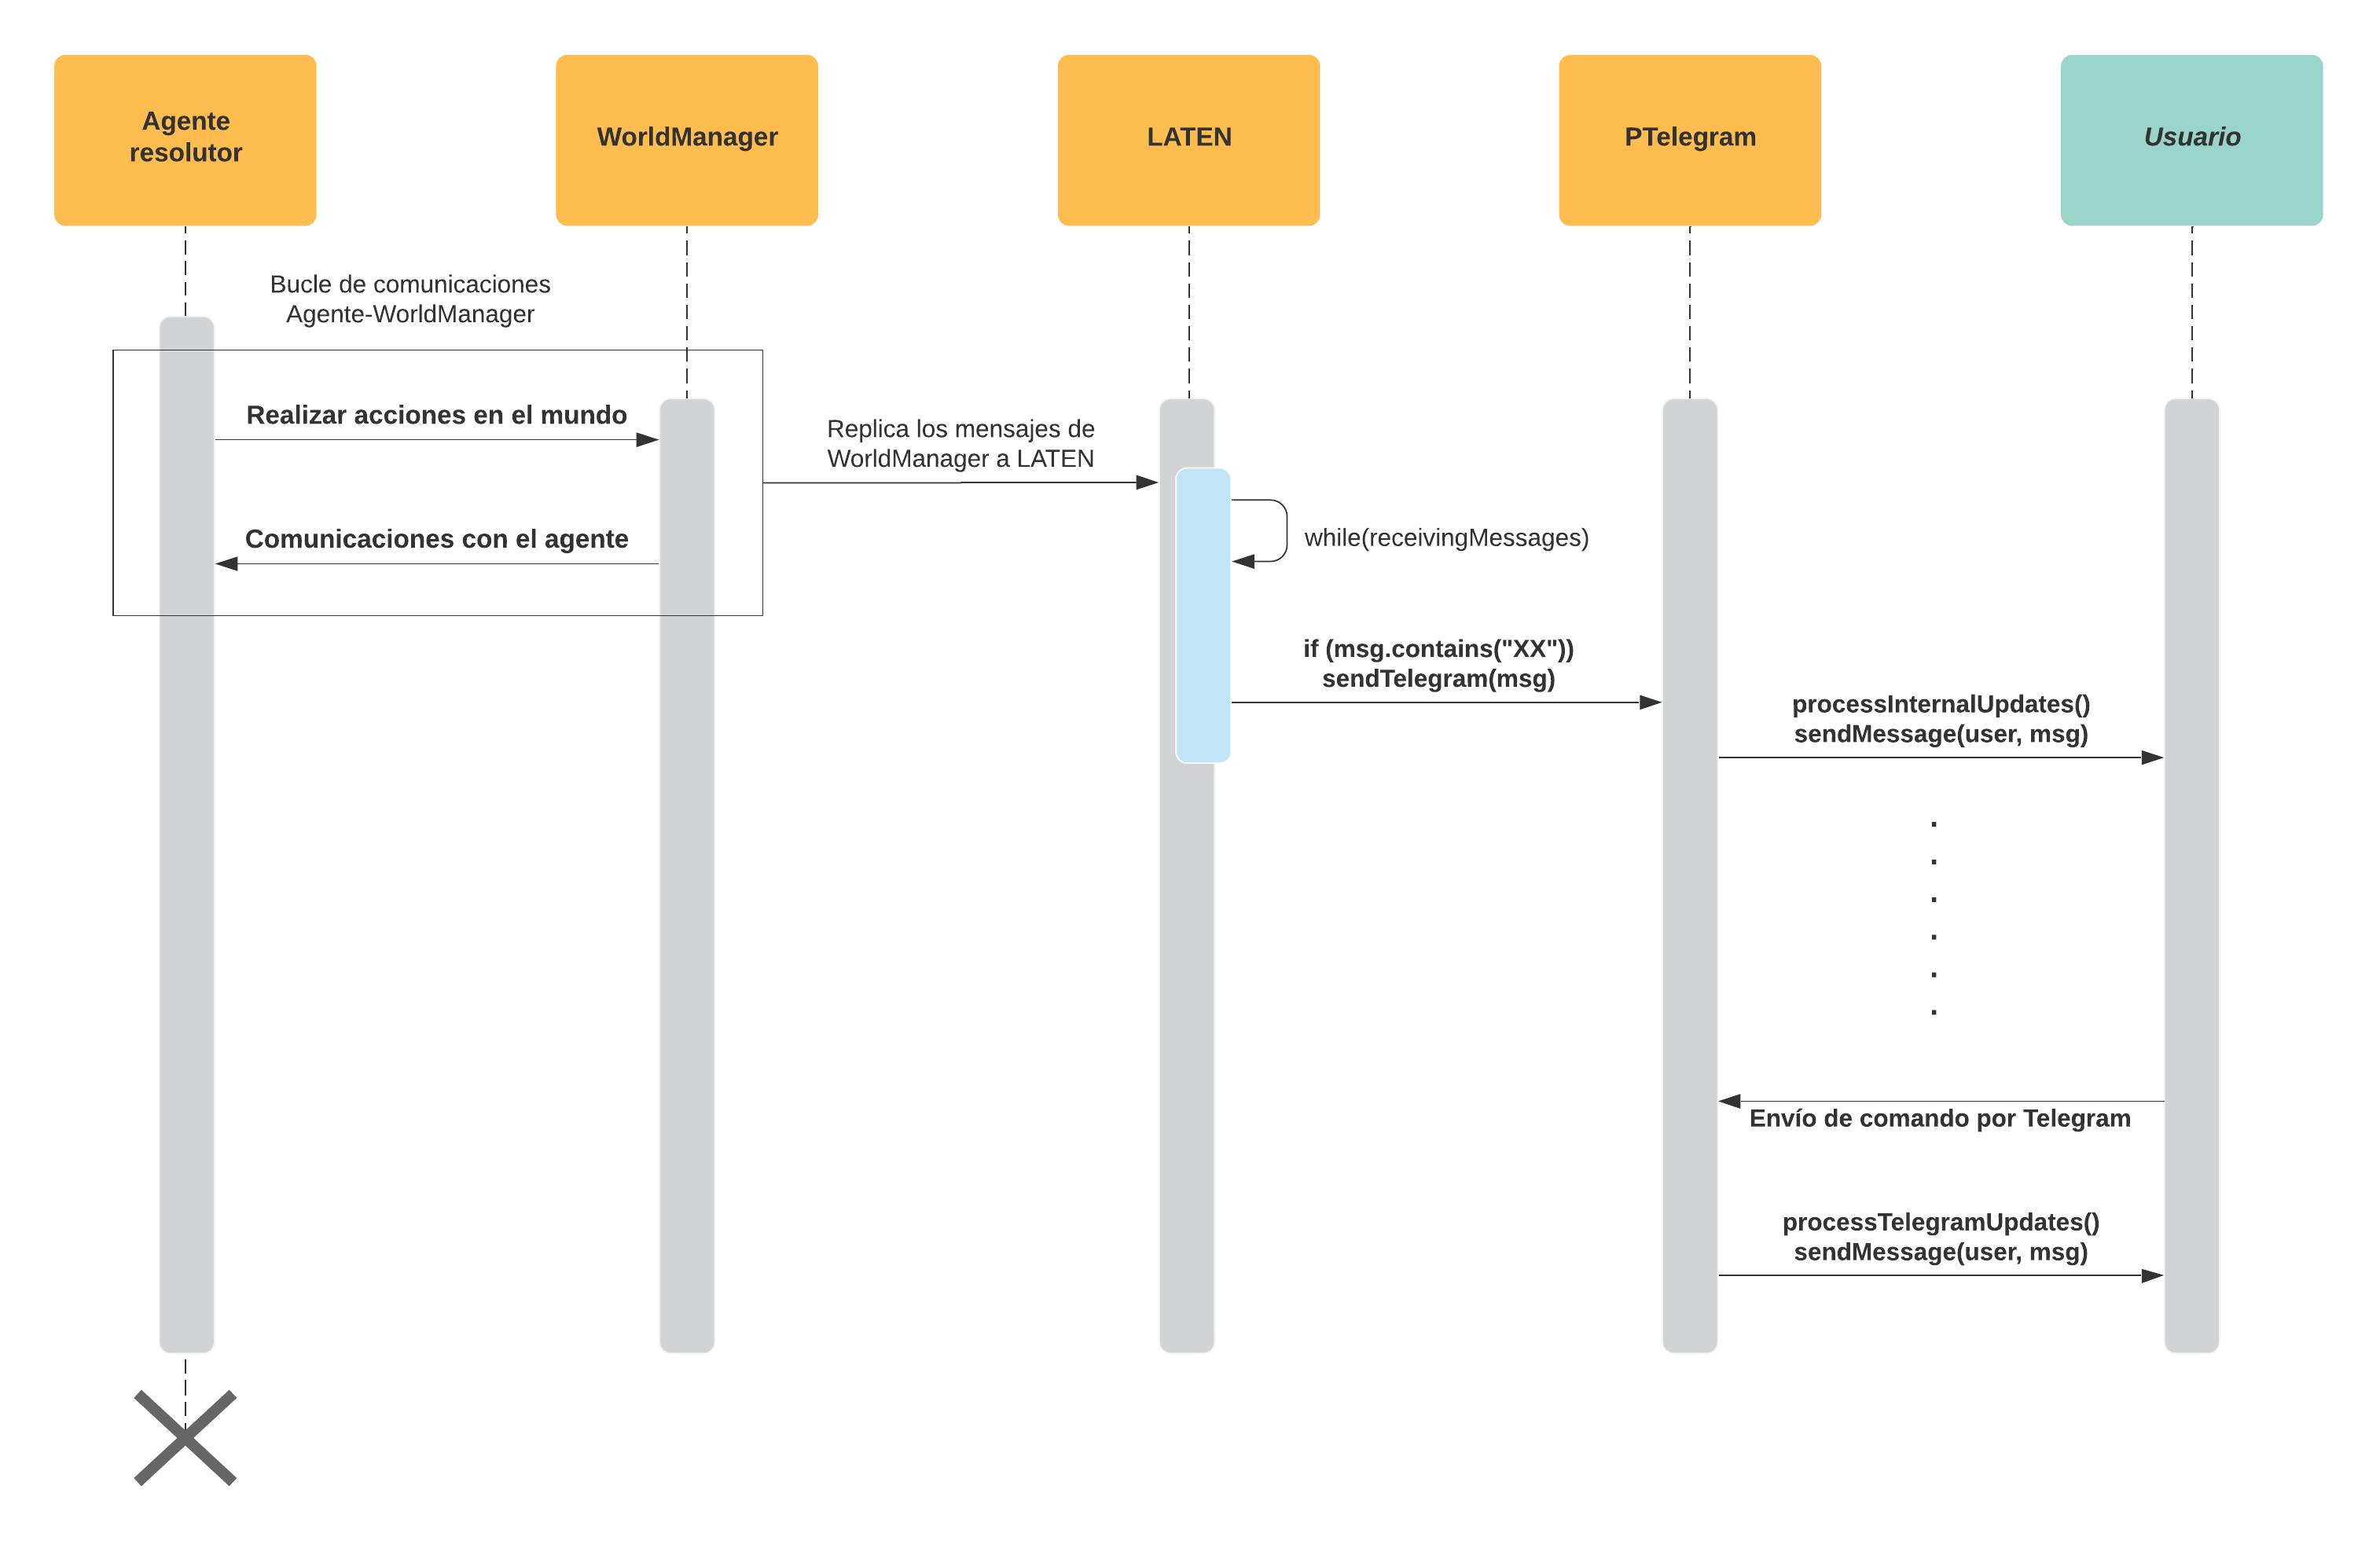
\includegraphics[width=1.1\textwidth]{logos/secuencia.png}\\[1.4cm]
\caption{Diagrama de secuencia de la red de agentes}
\label{img:secuencia}
\end{figure}

\section{Control de versiones: git y GitHub}

Además de las herramientas de desarrollo previamente mencionadas en las secciones de este capítulo, se han usado además otras dos herramientas para facilitar el desarrollo.\\

En concreto, para tener un control de las distintas versiones del proyecto, tanto a nivel de código como a nivel de documentación, he usado \textit{git} como tecnología de control de versiones y \textit{GitHub} para almacenar todo el proyecto.\\

El motivo de usar control de versiones surge desde el comienzo de mis estudios en el grado de Ingeniería Informática, donde se me presentó la necesidad de almacenar mis proyectos en un lugar seguro para evitar posibles pérdidas y además poder volver a versiones anteriores del código por si en algún momento del desarrollo algún componente falla, o se introduce algún fragmento de código que hace dejar de funcionar otra parte de manera estrepitosa.\\

Así, esa necesidad siguió evolucionando y siendo implementada de mejor manera por mi parte de lo largo del grado hasta llegar a este proyecto. Debido a la naturaleza del proyecto y que contiene algunos fragmentos de código sensibles que los alumnos de la asignatura no deberían tener accesibles, el repositorio de GitHub no se hará público, decisión que se tomó en consenso con el tutor de este proyecto.\\

No obstante, personalmente he mantenido de manera natural el control de versiones mediante el repositorio de GitHub como si fuese otra asignatura o proyecto más, a pesar de que no se hará público, al menos por ahora.\\

En la figura \ref{img:github}, se puede observar uno de los gráficos que provee GitHub. Este gráfico muestra el número de contribuciones realizadas en el repositorio en un periodo de tiempo determinado. A día tres de septiembre, se puede apreciar un nivel constante en las contribuciones al mismo desde el día cuatro de julio por parte de un único contribuidor \textit{(yo, el autor de este proyecto)}.

\begin{figure}[h]
\centering
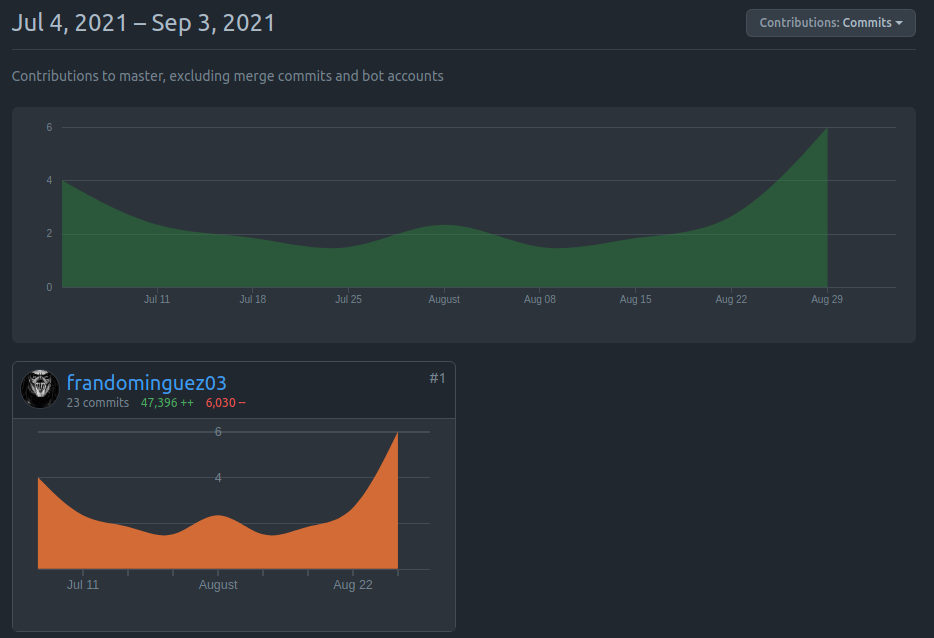
\includegraphics[width=0.9\textwidth]{logos/github.png}\\[1.4cm]
\caption{Gráfica de contribuciones del repositorio alojado en GitHub}
\label{img:github}
\end{figure}

	% Presupuesto

	% Conclusiones
	\chapter{Conclusiones y trabajos futuros}

A pesar de que durante la realización de la asignatura Desarrollo Basado en Agentes se adquirieron los conocimientos necesarios para llevar a cabo todas las prácticas de dicha asignatura, este proyecto ha servido para profundizar en muchos de esos aspectos y a su vez descubrir e investigar más de cerca las capas inferiores del desarrollo de agentes que no estaban visibles durante la asignatura.\\

Más concretamente, se ha comprobado de cerca cómo funcionan los comportamientos \textit{(behaviours)} de los agentes y otras especificaciones técnicas de JADE, como por ejemplo las colas de mensajes. Se han seguido durante el desarrollo del proyecto los estándares oportunos estipulados por la FIPA y se han intentado seguir los mismos patrones de diseños usados anteriormente por el creador de dichos proyectos, el profesor de la asignatura y tutor de este proyecto D. Luis Castillo Vidal.\\

Con respecto a los trabajos futuros, se podrían considerar las siguientes mejoras:\\

\begin{itemize}
	\item Mejorar el esquema de la base de datos
	\item Implementar funcionalidades en LATEN que puedan ayudar al profesor de la asignatura con las labores docentes
	\item Ampliar las funcionalidades de LATEN para los estudiantes
	\item Complementar LATEN con otros agentes de la plataforma para obtener mejores retroalimentaciones
\end{itemize}

Algunas de ellas estaban fuera del objetivo de este proyecto y otras simplemente no han sido planificadas, ya que en el marco del proyecto se contemplaban tareas más importantes para el desarrollo del mismo.

	% Trabajos futuros


	
	\newpage
	\bibliography{bibliografia}
	\bibliographystyle{plain}
	
\end{document}

